\thepage
\section{Introduction}

%- No collocation
%- Enterprise support
%- Version control, issue tracking

In recent years open source software solutions have become widely popular and frequently used in both scientific and enterprise use, which can be attributed to a number of factors, most importantly the ease of development and deployment of IT projects, improved cybersecurity and enhanced scalability \cite{pwcLeadingBenefitsOpensource2016}. This increases the contribution to open source projects from enterprises and individuals alike. Due to its nature, open source software projects are driven by community contributions, and depend heavily on active participation in all phases of the project.

Software development in a corporate environment usually follows a strict hierarchial structure, where each participant is given a precise position and responsibility, like project manager, scrum master, senior or junior developer, and employees do not tend to work outside of their assigned tasks and territories. The main purpose of maintaining software development structures is for the company to ensure that the outcome of the project is in accordance with the business objective, adheres to the pre-set quality criteria and it is completed in a given timeframe; in other words to asses the risks associated with the business objective of the software project \cite{surekaUsingSocialNetwork2011}. This is achieved by breaking down the developed software into smaller, less complex components, and grouping the developers into managable teams, where the communication is moderated between teams \cite{birdLatentSocialStructure2008}.

% Open-source software development propertie
As opposed to commercial software development, Free/Libre Open Source Software (FLOSS) projects usually do not follow an organizational hierarchy, and are usually self-organizing and dynamic \cite{birdLatentSocialStructure2008}. Issues, bugs and progress are tracked openly, and everyone is encouraged to contribute based on the current topics and expertise, but purely on a volunteering basis. The lack of access restriction to certain modules allows for much more spontaneous interaction between developers, which generate large, complex networks \cite{martinez-romoUsingSocialNetwork2008}. These complex networks can be seen as large social networks of developers based on collaboration.

% AUTHOR NAME HARDCODED HERE
Because contribution to FLOSS projects are voluntary, participants have a different motivation for taking part than in commercial software development. According to El Asir et al. \cite{elasriPeripheryCoreTemporal2017}, FLOSS participation can be motivated by internal and external factors. Internal factors include self-improvement, learning and contribution as a hobby or pass-time activity  \cite{alexanderharsWorkingFreeMotivations2002,yunwenyeUnderstandingMotivationOpen2003}, whereas external factors are motivated by marketing and demonstrating certain skills, thus increasing and improving employability \cite{alexanderharsWorkingFreeMotivations2002}.

% Summary of background literature and state of the art solutions
\section{Background and rationale}

\subsection{Collaboration in FLOSS projects}
% - FLOSS definition
% AUTHOR NAME HARDCODED HERE
Collaboration networks of open source software (OSS) have been a subject of many academic research. Raymond \cite{crowstonSocialStructureFree2005} has defined collaboration based on bug report interaction, and observed the collaboration network of 124 large-scale SourceForge projects. The generated networks have widely different centralization properties, but it was observed that larger sized projects tend to be more decentralized. The broad community roles contributors tend to take have been also identified in \cite{crowstonSocialStructureFree2005}, which have been coined as the \textit{onion model} in \cite{martinez-romoUsingSocialNetwork2008} (Figure \ref{fig:onion1}).

\begin{figure}
    \centering
    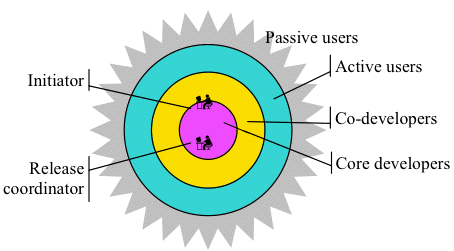
\includegraphics[width=0.6\textwidth]{figures/onion_model.png}
    \caption{Onion model of collaboration types in FLOSS projects \cite{crowstonSocialStructureFree2005}.}
    \label{fig:onion1}
\end{figure}

The onion model describes the types of participants in an OSS project as layers. The center represents the small group of core developers, who are responsible for the majority of contributions to the software. They are surrounded by a larger group of co-developers, whose main contributions are usually bug fixes reported by the active users. The passive users are usually the largest in numbers, who do not contribute or report any bugs. In a healthy FLOSS project, each layer of contributors are about one magnitude larger in numbers than the preceeding inner layer \cite{mockusTwoCaseStudies2002}.

% AUTHOR NAME HARDCODED HERE
El Asir et al. \cite{elasriPeripheryCoreTemporal2017} used a K-means classification to categorise project participants into a similar core-periphery structure (core, gray in-between area, and periphery) based on SNA metrics with a montly timeframe, and analysed how and why contributors transition between groups. They found that technical contributions like code commits and lines added have a much heavier impact on becoming a core developer as opposed to other activities, such as testing, reviewing and commenting.

% AUTHOR NAME HARDCODED HERE
A literature review conducted by McClean et al. \cite{mccleanSocialNetworkAnalysis2021} systematically analysed the state-of-the-art research of 46 scientific papers in the field of FLOSS social networks, and categorised them into three groups based on topic: structure, lifecycle and communication. They conclude, that the existence of core-periphery structure in OSS projects is well established in the field, which is also an indicator of a healthy FLOSS software. Regarding the lifecycle, generally the core development team does not change significantly over time, however, the project becomes more decentralised and distributed as it matures. A lack of research regarding temporal analyses were identified in the most current knowledge, which was suggested as a future research area in this field.

\subsection{Social network of Open-source projects}
In a larger FLOSS project, developers usually cannot understand every part of the project, therefore collaboration is required with eachother. The network created by the collaborators can be considered as a social network, because collaboration requires some kind of social interaction with eachother. Social network theory describes how social interaction patterns affect the individual behaviour \cite{martinez-torresGeneticSearchPatterns2012}. We can model an OSS project's social network as a graph, where nodes represent collaborators (developers, bug reporters, etc\dots) and edges represent the social interaction between them. In mathematical terms\dots TODO

The type of the social interaction determines the created network, therefore choosing the basis of collaboration can have a significant impact on the network structure. The common types of developer social networks (DSNs) are Version Control System-based (VCS-DSN), Bug Tracking System-based (BTS-DSN) networks and DNSs, that are purely based on social elements \cite{aljemabiEmpiricalStudyEvolution2018}. The VCS-DSN take the version control application as a source for network generation by recording collaboration based on co-edits of the same module, file or code section. Choosing the granularity can impact the precision of true collaborations represented in the network. Co-edits by multiple developers to a single module or file does not necessarily mean actual collaboration was required from the authors, as the parts edited could work functionally independent from eachother. By increasing the granularity to file sections (classes or functions within a single file) or even lines, we can be more certain, that coordination was required, but we risk leaving out semantically connected parts of the project \cite{joblinEvolutionaryTrendsDeveloper2017}. In contrast to VCS-DSNs' purely technical approach, the BTS-DSNs use semi-technical bases for connecting participants, such as comments on issues, bugs or reviews \cite{elasriPeripheryCoreTemporal2017}. These artifacts, although being tightly related to specific sections of the source code, allow for taking into account conversational elements as contribution. For example, participants, who do not contribute directly to the software source code, but actively review and comment, are also considered. Lastly, social networks of developers can be constructed on project participation, following, starring or through communication means like mailing lists. The technical aspect of collaboration is minimized in such DNSs, and they are more fit for project organization and communication analyses in FLOSS projects (mailing list vs file file edits vs line edits) \dots TODO


% \subsubsection{Global SNA metrics}

% \subsubsection{Local SNA metrics}

%\begin{itemize}
%   \item Relevant social aspects of OS projects
%   \item State of the art
%   \item Collaboration by coediting files
%   \item Contributors form dynamic social networks
%    \item Problem of analysing changes over time in a network
%   \item Other studies in this field...
%\end{itemize}

\subsection{OSS project success}
community maturity (\cite{linBlogCommunityDiscovery2007} in \cite{aljemabiEmpiricalStudyEvolution2018})

"Successful projects will likely have modular structure from the start or after refactoring as the source code grows larger and more unwieldy" \cite{antwerpEvolutionOpenSource2010}

success factors: Average Time Efforts, Number of Developers, Comments, Total Code Lines, Comment Ratio, Number of Rater \cite{yangHowMicrobloggingNetworks2013}
Truck Factor \cite{avelinoNovelApproachEstimating2016}


\section{Motivation of research problem and research questions}
Because there is a high dependency on the community in open source software projects, by understanding how contributions are included and what patterns emerge we can gain valuable insight into the project's current state and its trajectory. As stated before, SNA analysis of OSS have been extensively studied, but there is a lack of research regarding temporal models analyzing the lifecycle of a FLOSS project.

The goal of this paper is to fill in this gap by examining OSS project collaboration networks over time using SNA metrics. More specifically, one part of the research will focus on the evolution of such collaboration networks and comparing and contrasting these networks with the software outcome. The second part will focus on events during a project, and how it affects the developer collaboration. The research questions, which are broken down into subquestions, are as follows:

\begin{enumerate}
    \item \textbf{How does the temporal lifecycle information of a project influence its success?}
    
    \begin{enumerate}
        \item \textit{Based on temporal models of collaboration, is it possible to predict the outcome of the project?} Since it has been proven that the core collaborators do not change much over the course of the OS software development, our assumption is that any sudden or long-term change, that is not consistent with the other observed projects, can have a significant impact on the outcome (negative or positive alike).
        \item \textit{Can stages of a FLOSS project with a maturity model be observed?} As most OS software starts with a small collaborator basis and grows over time, it can be assumed, that each project goes through the same steps of open source maturity levels. On the other hand, it is also possible that due to the uniqueness of each project, no such stages are observable. 
    \end{enumerate}

    \item \textbf{How do major events in the project lifecycle change the collaboration network of the project?}
    \begin{enumerate}
        \item \textit{Do planned or foreseeable events change the collaboration structure?} Major software version releases can be considered foreseeable events of the project lifecycle, which could have an effect on the developer collaboration. For example, there might be a higher rate of interaction between contributors just before a new version is released to clear up the backlog of tasks. But it is also possible, that commit and change rates drop during this time, because the focus shifts to stability and testing instead of new features.
        \item \textit{How unforeseeable internal or external events affect FLOSS collaboration?} Sudden shocks to the project, such as an announcement of disinterest from major users of the software, discontinued enterprise support of the project, large-scale global events like the pandemic, or sudden employee firings can have significant effect on the core and periphery collaborators alike. By analysing the collaboration network before, during and after such changes, we might be able to recognise patterns, that regularly occur around these events.
    \end{enumerate}
\end{enumerate}

\subsection{Research methodology}
To find answers to the research questions above, first we build a repository analyzer tool, which mines collaboration data from FLOSS projects, generates static snapshot collaboration networks at each given time interval and calculates SNA metrics for each snapshot. Then these metrics can be aggregated over time, or plotted against time to discover changes in the network. The \texttt{git2net}\footnote{\url{https://github.com/gotec/git2net}} \cite{goteAnalysingTimeStampedCoEditing2019} Python library provides the necessary tools to mine any project repository that uses git version control. It also incorporates temporal network generation capability, which can be used as a source for creating static collaboration networks aggregated over a given period of time.


We apply a hybrid methodology of qualitative and quantitative research. First, as part of the qualitative research, we choose a small number of repositories to be analyzed. We observe the number of connected components, centrality, number of nodes and mean degree SNA metrics in order to discover the core and peripherial collaborators over the project lifecycles. The basis of collaboration, due to the unavailability of other means of communication, is coediting files. Based on the state of the art research in this field, file coediting proves to be an effective and easy way to represent collaboration between developers.

After discovering the collaboration structure over time, we will match the breakpoints and unexpected spikes or troughs to events within the lifespan of the project. We expect that the key SNA metrics will show a periodicity around planned releases and other reoccurring events (e.g. holiday season). Outstanding values without reoccurrence, on the other hand, are more likely to be consequences of unexpected events. In these cases, it should be observed whether the network is capable of reorganizing itself, or does the event leave a permanent mark on the collaboration structure. A categorization of unexpected events and the level of impact each category has should be observed.

For the quantitative research to be conducted, we will gather a large set of repositories along with major events in its lifecycles. We will then run the miner for all repositories, and with the findings of the qualitative research, we will try to detect all major events and their type (planned or unexpected). We will utilize the \texttt{ruptures} \footnote{\url{https://github.com/deepcharles/ruptures}} library to detect changes in the continuous SNA metrics. If the model is capable to accurately recognise events, then we can also apply it on any repository to detect changes, which will allow us to discover changes in the collaboration network that are not related to publicly known events or releases.

% Quantitative research
% \begin{itemize}
%     \item Composing a large set of repositories (different sizes, properties) with their success or failure
%     \item Gathering major events for the repositories (version releases, external events, global events)
%     \item Detecting past changes automatically based on changes in measured statistics
%     \item How do changes and reoccurring patterns match the events?
%     \item What structures can be noticed before a major success or failure of a project?
% \end{itemize}


\section{Gitminer implementation}
To find answers to the research questions, we implement an analysis tool to mine and analyze project repositories, which allows us to generate collaboration networks and network metrics for the analysed projects.

\subsection{\texttt{git2net} miner}
The process begins with the project mining. After cloning the repository, the \texttt{git2net} \cite{goteAnalysingTimeStampedCoEditing2019} library is used to collect data related to commits. Specifically, who is the author of each commit, which files were modified (created, edited, deleted) with the commit, and when was the commit created. Additionally, the lines edited by the author within each commit are collected separately, allowing for a more fine-grained collaboration network generation if necessary. The results are collected into an \texttt{sqlite} \footnote{\url{https://www.sqlite.org/index.html}} database file's \textit{commits} and \textit{edits} tables.

The \texttt{git2net} mining process by default collects all the commits throughout the project's lifecycle. However, the processing time of each commit differs based on the number of edits, the affected number of files and the file types as well, which makes collecting certain commits very resource-intense and time-costly. Therefore, we exclude every commit, which contains more than 100 file modifications, during each repository mining using the \textit{max\_modifications} parameter. As observed by Gote et al \cite{goteAnalysingTimeStampedCoEditing2019}, this exclusion criteria does not affect significanly the generated network, because they are mostly merge commits or project restructurings, which do not mark any true collaboration effort between developers. During the data mining in certain repositories, we encountered commits, that were not mineable with this method and the mining process halted, presumably due to processing error because of binary file changes in these commits. We also excluded these commits from our data mining process.

This exclusion criteria resulted in an average of 3\% of commits excluded in all repositories subject to our analyses, with the highest excluded commit rate being 20\%.

\subsection{\texttt{repo\_tools} miner} 

We use the \texttt{repo\_tools} \footnote{\url{https://github.com/wschuell/repo\_tools/}} Python library to query the Github API for additional repository data extraction, such as:

\begin{itemize}
    \item Releases
    \item Tags
    \item Issues
    \item Stars and followers
\end{itemize}

The mining output is also stored in a \texttt{sqlite} relational database, which is queried later on during the analysis. 

% - what do we want to achieve with the gitminer
%  - generate networks of collaboration
%    - what should be the basis of collaboration
%  - filter for time
%  - generate statistics

\subsection{Data preprocessing}

The collaboration networks with the \texttt{git2net} library connect the authors to their edited files using only file and author names instead of IDs. This creates an issue when generating the networks, because authors with the same name will show up as one node, and they will be connected to the files they touched combined. Furthermore, authors that change their displayed name ('author\_name' field in the mining database) or log in from diferent accounts, where they have different names, will show up as multiple nodes instead of a single vertex.

We utilize the \texttt{gambit} \cite{goteGambitOpenSource2021} rule-based disambiguation tool to resolve the author names. Furthermore, the created networks have issues when the node names contain special characters or spaces. Therefore, after disambiguation, we replace every unique author name with its ID number.

As the files are also labelled by their filename property in the network outputs, the same filenames but in different folders are also displayed as single nodes. In order not to create false collaborations, we simply remove the files from the network with filenames, that occur more than once in all the repository subdirectories. We argue that this does not remove any significant collaboration data, since most files sharing their name with other files are technicaly files, like \texttt{\_\_init\_\_.py} for a Python project.

\subsection{Collaboration networks}

When creating a DSN from the mined data, we have multiple methods at hand. The \texttt{git2net} library provides its own co-editing network function, which returns a temporal network of collaborators. This uses the co-authorship algorithm developed by Gote et. al. \cite{goteAnalysingTimeStampedCoEditing2019}, however, we would like to have more control over the network generation method, such as simple file-based co-authorship in order to customize the network for our needs, like weighing each relation or generating undirected graphs.

\subsubsection{Temporal bipartite network}
As a first step, we generate a temporal bipartite network of authors and their edited files with the \texttt{git2net} built-in \textit{get\_bipartite\_network} method. A temporal network is a \texttt{pathpy} \footnote{\url{https://www.pathpy.net/}} graph object, which contains a collection of timestamped graphs of a single network at each point in time within the observed timeframe. Such a snapshot $S_t = (U, V, E_t)$, where $U$ is the set of authors, $V$ is the set of files and $E_t$ is the set of file edits as edges at $t$ timestamp. By connecting the authors, who touched the same files, and removing the nodes representing the edited files (converting the bipartite network to a regular network), we can observe the evolution of the collaboration over time, represented in Figure \ref{fig:temporal net}.

\begin{figure}
    \centering
    \begin{subfigure}{0.3\textwidth}
        \centering
        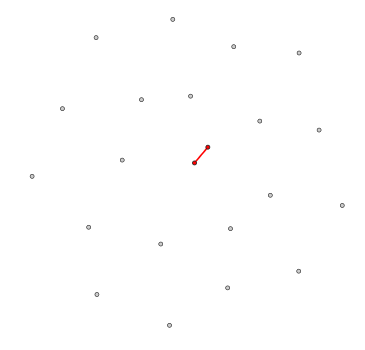
\includegraphics[width=0.92\textwidth]{figures/temporal/0.png}
        \caption{}
        \label{fig:temporal net A}
    \end{subfigure}
    \hfill
    \begin{subfigure}{0.3\textwidth}
        \centering
        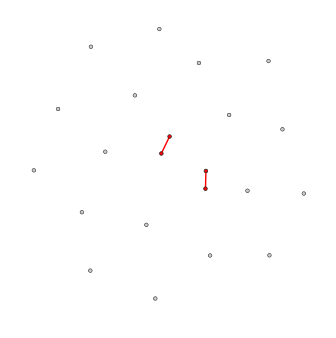
\includegraphics[width=0.92\textwidth]{figures/temporal/1.png}
        \caption{}
        \label{fig:temporal net B}
    \end{subfigure}
    \hfill
    \begin{subfigure}{0.3\textwidth}
        \centering
        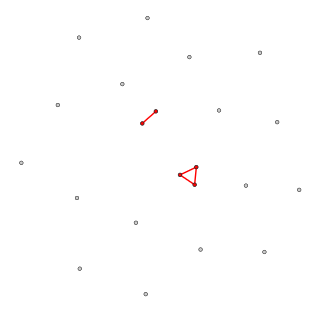
\includegraphics[width=0.92\textwidth]{figures/temporal/2.png}
        \caption{}
        \label{fig:temporal net C}
    \end{subfigure}
    \hfill
    \begin{subfigure}{0.3\textwidth}
        \centering
        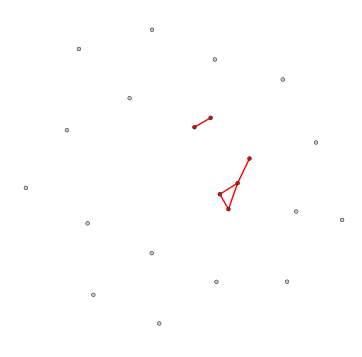
\includegraphics[width=0.92\textwidth]{figures/temporal/3.png}
        \caption{}
        \label{fig:temporal net D}
    \end{subfigure}
    \hfill
    \begin{subfigure}{0.3\textwidth}
        \centering
        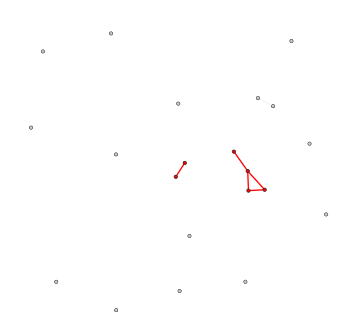
\includegraphics[width=0.92\textwidth]{figures/temporal/4.png}
        \caption{}
        \label{fig:temporal net E}
    \end{subfigure}
    \hfill
    \begin{subfigure}{0.3\textwidth}
        \centering
        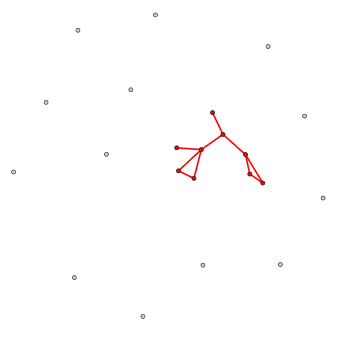
\includegraphics[width=0.92\textwidth]{figures/temporal/5.png}
        \caption{}
        \label{fig:temporal net F}
    \end{subfigure}
    \caption{Sequential snapshots of the \texttt{networkx} collaboration network with a moving time-window of 30 days and 7-day steps.}
    \label{fig:temporal net}
\end{figure}

Although a temporal network preserves the time aspect of the graph by the edges being tied to the time dimension of the graph, calculating network metrics like centrality on such networks is infeasible. Visualization also proves to be difficult in representations where animation is not possible. Therefore, we aggregate the bipartite network over a given timeframe into a static network. All nodes within the temporal net are preserved, and all directed edges are added to the network with the edge weight representing how many times that author edited the file.

\subsubsection{Static networks}
The generated static weighed bipartite network looses its time-varying component, but now we are able to manipulate and calculate complex statistics over it. Figure \ref{fig:bipartite} is an example of such a network. As a next step, we convert the the bipartite network into an authors' network by removing the nodes representing files.

\begin{figure}
    \centering
    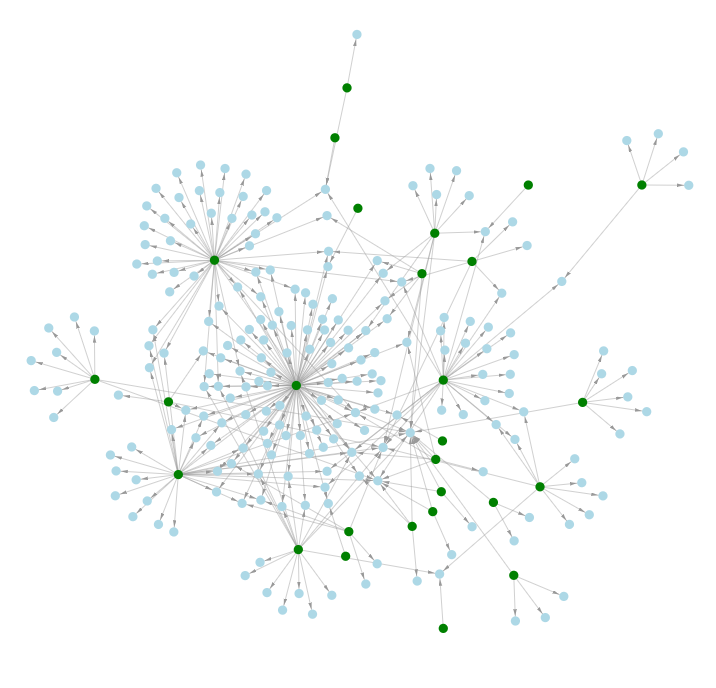
\includegraphics[width=0.65\textwidth]{figures/bipartite.png}
    \caption{A bipartite network of authors (green) and edited files (light blue) in the \texttt{pandas} project within the timeframe 31/01/2021 and 15/02/2021}
    \label{fig:bipartite}
\end{figure}

We have multiple methods to convert the directed and weighted bipartite network into a projection of authors. We could simply remove the files and connect each author, that worked on the same file, however, the end result would be an unweighted graph. This would falsely show, that all collaborations are weighed equally, which is clearly not the case, as multiple continuous edits on the same file from both parties should represent a stronger collaborative connection. Therefore, firstly we implement the Weighted One-Mode Projection (WOMP) method \cite{stramWeightedOneMode2017}, The WOMP method converts the bipartite network $G(A,F,E)$, where $E$ is the edge list containing tuples $(a_i,f_i,w_{ij})$, and $w_{ij} \in E$ is the weight between author $a_i \in A$ and file $f_i \in F$. With this notation, a weighted directed edge can be calculated for any $a_a, a_b \in A$ as follows:

\[ w_{ab}^{A \rightarrow A} = \sum_{j=1}^m \frac{w_{aj}}{W_a^F}, \]

where $W_a^F$ is the sum of all outgoing edge weights from author $a$ to all files $F$ denoted as $W_a^F = \sum_{i=1}^n w_{ai}$. This creates a bidirectional weighted collaboration network between authors $a_1$ and $a_2$, where the weight $w_{12}$ represents the relative collaboration effort of $a_1$ towards $a_2$ compared to all the other developers $a_1$ has collaborated with. Conseqently, every edge is in the rage $[0,1]$ in the resulting WOMP network.

A disadvantage of the WOMP method is, that the generated collaboration network is bidirectional, meaning if there was any common authored files between $a_1$ and $a_2$, then there will be both $w_{12}$ and $w_{21}$ connecting them. To simplify the network, we want to generate an authors network, where the edges are undirected. For this, we are using the weighted Jaccard method on the files-authors bipartite network:

\[ w_{ab} = \frac{\sum_{f \in F}min(f_a, f_b)}{\sum_{f \in F}max(f_a, f_b)}. \]

For each file $f$ that $a_1$ and $a_2$ authors touch, we sum up the minimum and maximum weights the authors have towards each file, then we divide the sum of minimums with the sum of maximums. This results in the undirected author-author network with edge weights in range $[0, 1]$. By default, this method removes isolated contributors, who do not collaborate with eachother, but are actively editing the files. We add these nodes manually. Figure \ref{fig:jaccard} shows the final author network.

\begin{figure}
    \centering
    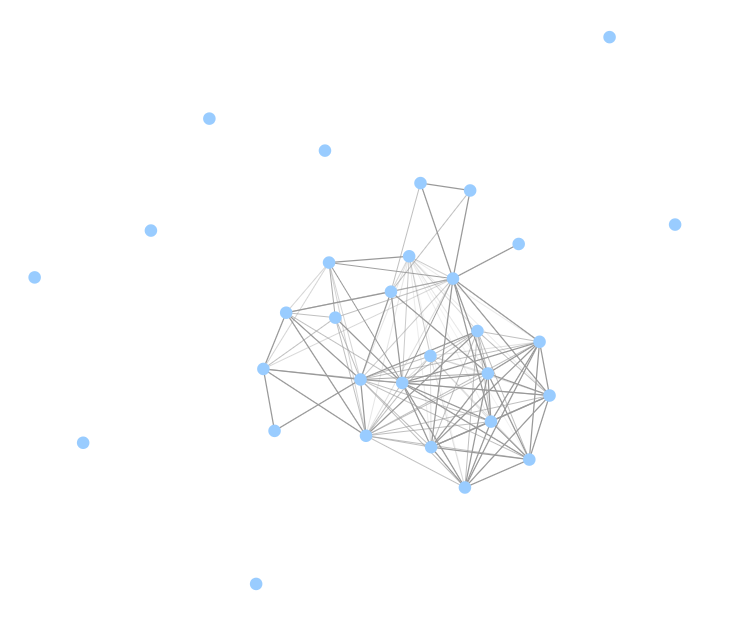
\includegraphics[width=0.9\textwidth]{figures/jaccard.png}
    \caption{Weighted Jaccard similarity collaboration network of \texttt{pandas} generated from the bipartite network in Figure \ref{fig:bipartite}.}
    \label{fig:jaccard}
\end{figure}

\subsection{Core and periphery, centralization}
A critical part of the OSS software projects is the existence of core and periphery developers. It has been observed, that in each FLOSS project there are a small number of developers, who provide the vast majority of development effort into the project. It has been also established, that the members of core developers do not change substantially during the project's lifecycle. However, there was no effort on whether there is a change in the collaboration pattern, especially before, during or after a major lifecycle event. Therefore, we make efforts identifying the core developer network to observe these changes.

\subsubsection{Degree centrality}
\label{sec:deg_centrality}

We use the degree centrality of each node (i.e. developer) to identify the core members. Degree centrality of a node is the fraction of all possible nodes it is connected to. We can calculate it by dividing the degree with $n-1$, where $n = |G|$ the number of nodes within the network. Since the core developers contribute the majority of commits and edits of the project, they are expected to be connected with more nodes. Joblin et. al. \cite{joblinClassifyingDevelopersCore2016, joblinEvolutionaryTrendsDeveloper2017} have also identified degree centrality as the best predictor of core developers. In cases, where binary classification of core or periphery is needed, we assign developers to the core network if their degree centrality score is in the top 20th percentile, otherwise they are considered as periphery. We also take note, that this method does not consider the weighted edges, only the number of edges (degree) a node has. Although this method could be refined to consider the node degree weighted with the edges, we argue that this could lead to invalidity. In case of two developers, who only contributed to one file, they will be represented with a strong connection and would receive a high weighted degree value, whereas a core contributor, who edits many files, can have many weak connections but these might not add up to one strong connection of the two isolated developers when weighted with the edge weights. It is clear, that a developer with many connections, regardless of the strength of the collaboration, should be considered core. Figure \ref{fig:degree centrality} shows two examples for degree centrality within a collaboration network. In the figure, darker colors represent a higher degree centrality value. The  highlighted nodes are in the highest 20th percentile of degree centrality, classifying as members of the core developers. We can observe in both one-month periods, that \texttt{pandas} is much more decentralized, whereas \texttt{curl} is largely dependent on one developer.

\begin{figure}
    \centering
    \begin{subfigure}{0.49\textwidth}
        \centering
        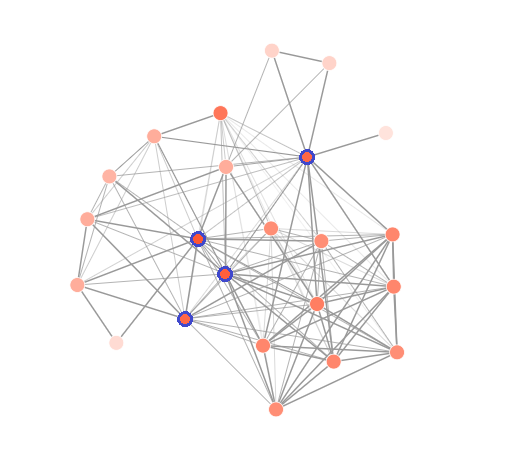
\includegraphics[width=0.98\textwidth]{figures/degree_centrality.png}
        \caption{Pandas}
        \label{fig:centrality a}
    \end{subfigure}
    \hfill
    \begin{subfigure}{0.49\textwidth}
        \centering
        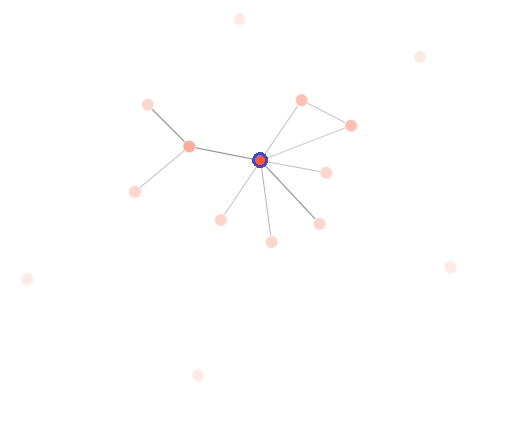
\includegraphics[width=0.98\textwidth]{figures/degree_centrality_curl.png}
        \caption{Curl}
        \label{fig:centrality b}
    \end{subfigure}
    \caption{Degree centrality within the \texttt{pandas} and \texttt{curl} projects' collaboration networks. }
    \label{fig:degree centrality}
\end{figure}

\subsubsection{Degree centralization}

The degree \textit{centrality} can be calculated for every node, however, through our analysis we would also like to measue a global \textit{centralization} metric, which is applicable to the whole network. As suggested by Crowston and Howison \cite{crowstonHierarchyCentralizationFree2006}, we calculate the degree \textit{centralization} by summing the differences between the maximum and each node's degree \textit{centrality}. 

\[ C_D(A) = \frac{\sum_{i=1}^n(C_d(a*)-C_d(a_i))}{H}, \]

where $C_d(a)$ is the degree \textit{centrality} of an author $a$, $a*$ is the author with the highest degree \textit{centrality} value, and $n$ is the number of authors in the collaboration network $A$. The value $H$ is for normalizing the sum by dividing by the theoretical maximum \textit{centralization}. Since the \textit{centrality} values are already in the range $[0, 1]$, we only need to normalize for the network's size. We get the highest centrality score with a star graph, where each node is only connected to a single central node, which has exactly one edge to all other nodes. The central node has a centrality of 1 in this case, whereas all the other $n-1$ nodes have $C_d(a) = \frac{1}{n-1}$. This means that in case of a star graph:

\[ H = (n-1) (1-\frac{1}{n-1}) = n-2. \]

Within certain timeframes, when a project is inactive, it could happen, that the network contains 2 nodes or less. We define $C_D(A) = 0$ if $|A| = n <=2$. The resulting output will always have a value in $[0, 1]$, where 1 means a completely centralized network (star graph) and 0 means a completely decentralized network. It is important to emphasize that a centralization score of 0 does not necessarily mean that there is no collaboration and every developer is isolated. Rather it means that each developer is co-authoring with just as many authors, as the others do.

% - Gini coefficient

% - \cite{klugUnderstandingGroupDynamics}

\subsubsection{Clustering coefficient}
\label{sec:clustering}

While centralization helps us describe the centralness of the network and how much it is centered around a single, or a small number of developers, it does not help us describing the structure of the network in more detail. Our goal is to gain an understanding of also the modularity of our network, meaning how much developers tend to cluster together \cite{joblinEvolutionaryTrendsDeveloper2017}. We expect that authors form smaller clusters, which are more tightly connected together, and these clusters have somewhat weaker ties to other clusters. This builds on the assumption that the social network of the software follows the modules which build up the software itself, thus authors of a specific function should also cluster together within the network \cite{conwayHowCommitteesInvent1968, joblinEvolutionaryTrendsDeveloper2017}. To measure this "clusteredness", we calculate the \textit{local clustering coefficient} for each node.

\begin{figure}
    \centering
    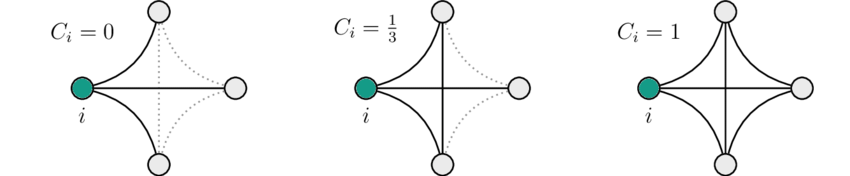
\includegraphics[width=1\textwidth]{figures/loc_clust_coeff.png}
    \caption{The local clustering coefficient demonstrated on an unweighted network of 4 vertices \cite{jedrzejewskiRoleComplexNetworks2016}.}
    \label{fig:loc clust coeff}
\end{figure}

The \textit{local clustering coefficient} quantifies on a scale $[0, 1]$ how likely it is that a node's neighbours are also neighbours. We use the number of how many triangles (also called clique, triplet) is every node a part of. This is illustrated for unweighted networks on Figure \ref{fig:loc clust coeff} with the formula:

\[ C_i = \frac{2T(i)}{deg(i)(deg(i)-1)}, \]

where $T(i)$ is the number of triangles through node $i$ and $deg(i)$ is the degree of i. However, in a weighted network we also have to consider the edge weights, since it is easy to see that a clustering coefficient of 1 with also the maximum weighted edges in a triplet does not represent the same clustering as being connected with a weak links. We expect weaker links connecting larger clusters, whereas stronger links within each cluster. Therefore, we use geometric averaging of the subgraph edge weights (as implemented by the \texttt{networkx}\footnote{\url{https://networkx.org/documentation/stable/reference/algorithms/generated/networkx.algorithms.cluster.clustering.html}} library \cite{onnelaIntensityCoherenceMotifs2005}):

\[ c_i = \frac{\sum_{jk}(\hat{w}_{ij}\hat{w}_{ik}\hat{w}_{jk})^{1/3}}{deg(i)(deg(i)-1)}. \]

The $\hat{w}_{ij}$ represents the normalized weight of edge $e_{ij}$ over the maximum weight in the network.

\subsubsection{Hierarchy}
\label{sec:hierarchy}

The degree centrality and the clustering coefficient are in themselves able to express meaningful aspects of the developer social network, however, by combining the two metrics, we can also assess how hierarchical the network is. In a scale-free social hierarchical network (such as the collaboration network), nodes tend to cluster around a single or a few hubs, which are more likely to have weak connections to other hubs \cite{ravaszHierarchicalOrganizationComplex2003, joblinEvolutionaryTrendsDeveloper2017}. The nodes within these formed groups are relatively stronger than the connections connecting the hubs, but they are less likely to connect to nodes outside of their group. Therefore in a hierarchical network, the hubs have a high degree number and a low clustering coefficient, whereas the group members clustering around the hubs have a high clustering coefficient, but low degree numbers.

We can visualize the degree of hierarchy by plotting each node's  clustering coefficient against the number of degrees, shown in Figure \ref{fig:hierarchy}. In hierarchical networks, the plotted linear regression trendline will decrease steeply, as there is a negative correlation between the degree and clustering coefficient. In networks, where this cannot be observed, the trendline stays flat, meaning these two metrics are independent from eachother and the structure is not hierarchical. To measure the hierarchical level numerically within a network, we take the trendline's slope, which is $\beta_1$ in the $y=\beta_1x + \beta_0$ general linear regression equation.

\begin{figure}
    \centering
    \begin{subfigure}{0.49\textwidth}
        \centering
        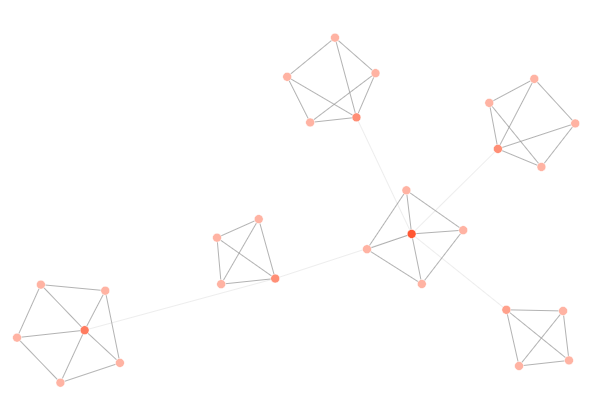
\includegraphics[width=0.98\textwidth]{figures/hierarchical.png}
        \caption{Highly hierarchical network}
        \label{fig:hierarchical}
    \end{subfigure}
    \hfill
    \begin{subfigure}{0.49\textwidth}
        \centering
        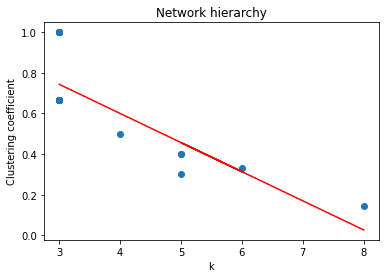
\includegraphics[width=0.98\textwidth]{figures/hierarchy_plot.png}
        \caption{Network hierarchy}
        \label{fig:hierarchy plot}
    \end{subfigure}
    \caption{Hierarchical network and its corresponding degree number vs clustering coefficient plot.}
    \label{fig:hierarchy}
\end{figure}

In every network isolated authors can be observed, who are only working on files that noone else has edited (in the given timeframe). These nodes can skew the hierarchy score, because an isolated node's degree and clustering coefficient are by definition 0, which disproportionately makes the trendline much flatter. Therefore, we remove the isolated nodes from the network. If the network only contains isolated nodes, and there is no linear regression to be calculated, we set the hierarchy value to 0.

\subsection{Project measures}

One of our assuptions is that the collaboration network structure changes depending on the project's lifecycle. In order to discover cause and effect relationships between the network structure and project lifecycle, we gather basic project metrics to pinpoint the time and date of events, as well as the effort required within the project. We achieve this by gathering the dates of each release, and the quality and relative stress is measured by the issues within the project (create and close times).

\subsubsection{Release and release measures}

To measure the network changes around releases, first we collect the list of releases for the given project. Our goal is to gather the version number of each release, as well as the dates they were released. There are two relevant APIs regarding the release version numbers: GitHub releases and Git tags. Tags are marked and annotated commits supported by Git, therefore other projects, that are not on GitHub can also have tags. \textit{Tags} are most commonly used to mark new release versions, but they can also be used to annotate other information, such as release editions or milestones. On the other hand, a \textit{Release} is a high-level GitHub concept, which allows the project organizers to announce Git tags as project releases by adding a version number, release notes and binary artifacts \cite{olsonReleaseYourSoftware2013}. A commit, that represents a new GitHub release, must be tagged, but a tagged commit does not necessarily need to be a new GitHub release.

\begin{figure}
    \centering
    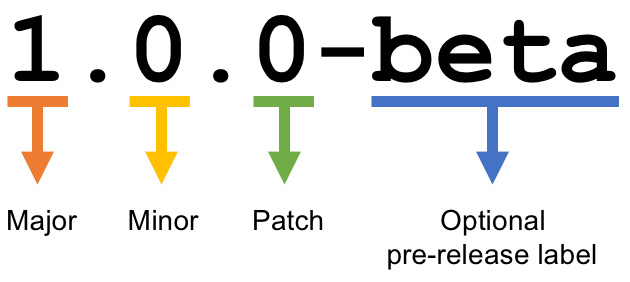
\includegraphics[width=0.5\textwidth]{figures/semantic-versioning.png}
    \caption{Semantic versioning. Figure source: \cite{mariogripSemanticVersioningUT2018}.}
    \label{fig:semver}
\end{figure}

Throughout our analysis, we use the tags as indicators of a new release, because there could be new versions of a software, that are not released publicly, and therefore do not have a GitHub release. Furthermore, GitHub only announced the Releases workflow in 2013, when the release versioning by Git tags was already a common practice. This means, that releases before 2013 can only be analysed via the repository tags.

Most large-scale OSS proejcts follow the semantic versioning convention, but only to a certain extent. The majority of tags follow the major-minor-patch (also known as breaking-feature-fix) semantic version naming convention in the format of X.Y.Z, where X is the major number, Y is the minor number, and Z is the patch number \cite{preston-wernerSemanticVersioning}. At the end, optionally pre-release and build data can be marked, for example: \textit{1.11.6-pre}. The major number signifies an API-breaking change compared to the previous release, meaning backwards compatibility is not guaranteed for depending applications. Minor releases add new features, but compatibility is ensured with the older version. Patch releases usually handle bugs and security updates within the package.

During the network analysis, we expect the network measures to change around a release, but it is also expected, that a larger release, that required more collaboration, will have a greater impact, while smaller changes have smaller or no impact at all. The issue with the semantic versioning and release names is that there are no constraints, which would enforce a strict version naming, and it is entirely up to the developers to set the tag names. This leads to inconveniences when measuring collaboration effort through release version number, because a patch might require more collaboration effort than a minor release, and a minor release within one project could require significantly more teamwork than in another. Furthermore, tag names can be inconsistent, and there could be version numbers, that do not adhere to the major-minor-patch naming convention at all (e.g. test releases, or releases like 'latest-release-v11'). The possibility to add extra information at the end of tag names, like \texttt{-beta} or \texttt{rc} further complicates tracking the collaboration effort, because the majority of collaboration effort might happen before the \texttt{rc} version, or it might happen after it. As it can also be seen in Table \ref{tab:releases}, the \texttt{v0.14.0rc1} tag contains more modifications than the final \texttt{v0.14.0} version, whereas the \texttt{v1.2.0rc0} only contains a small fraction of modifications compared to \texttt{v1.2.0}.

\begin{table}
    \centering
    \resizebox{\textwidth}{!}{%
        \begin{tabular}{| c | c | c | c | c | c | c | c | c |}
            \hline
            \textbf{Index} & \textbf{Name} & \textbf{Tag name} & \textbf{Created} & \textbf{Type} & \textbf{Modifications} & \textbf{Lines added} & \textbf{Lines removed} & \textbf{Total change} \\
            \hline \hline
            0 & Pandas v0.13.0 & v0.13.0 & 2013-12-30 17:02:51 & unknown & 20031 & 1.665357e+09 & 1.624343e+09 & 3.289700e+09 \\
            1 & Pandas v0.13.1 & v0.13.1 & 2014-02-03 04:52:01 & patch & 836 & 2.231875e+06 & 2.349833e+06 & 4.581708e+06 \\
            2 & Pandas v0.14rc1 & v0.14.0rc1 & 2014-05-16 22:28:09 & minor & 1861 & 2.251189e+07 & 2.050846e+07 & 4.302035e+07 \\
            3 & v0.14.0 final & v0.14.0 & 2014-05-30 11:47:40 & unknown & 318 & 3.220804e+06 & 5.314470e+05 & 3.752251e+06 \\
            4 & v0.14.1 final & v0.14.1 & 2014-07-10 23:46:19 & patch & 720 & 1.660133e+06 & 3.796690e+05 & 2.039802e+06 \\
            5 & v0.15.0 Pre-release & v0.15pre & 2014-09-07 12:52:01 & unknown & 826 & 1.028779e+07 & 2.458664e+06 & 1.274645e+07 \\
            \dots & \dots & \dots & \dots & \dots & \dots & \dots & \dots & \dots\\
            66 & Pandas 1.1.5 & v1.1.5 & 2020-12-07 11:42:10 & patch & 2167 & 4.251057e+06 & 4.611365e+06 & 8.862422e+06 \\
            67 & Pandas 1.2.0rc0 & v1.2.0rc0 & 2020-12-08 12:31:44 & minor & 41 & 1.060500e+04 & 8.850000e+02 & 1.149000e+04 \\
            68 & Pandas 1.2.0 & v1.2.0 & 2020-12-26 13:47:00 & unknown & 683 & 5.782570e+05 & 2.989310e+05 & 8.771880e+05 \\
            69 & Pandas 1.2.1 & v1.2.1 & 2021-01-20 11:21:02 & patch & 1306 & 1.864636e+07 & 9.228629e+07 & 1.109326e+08 \\
            70 & Pandas 1.2.2 & v1.2.2 & 2021-02-09 10:55:19 & patch & 844 & 6.783283e+06 & 1.827142e+07 & 2.505470e+07 \\
            71 & Pandas 1.2.3 & v1.2.3 & 2021-03-02 09:43:36 & patch & 959 & 1.002189e+07 & 5.783745e+06 & 1.580563e+07\\
            72 & Pandas 1.2.4 & v1.2.4 & 2021-04-12 15:59:13 & patch & 289 & 3.402820e+05 & 1.704960e+05 & 5.107780e+05\\
            \hline
        \end{tabular}} \\
    \caption{Releases collected information.}
    \label{tab:releases}
\end{table}

In order to have a more fine-grained measure of how much effort a release required (besides the semantic versioning), we measure the number of lines added and lines removed in that release. This is calculated by adding up each commit's 'total lines added' and 'total lines removed', which was authored after the previous release but up to and including the current release tag's commit. The total change of lines for a release is simply the sum of lines added and lines removed, which are provided by the \texttt{git2net} miner. The miner also provides the number of modifications for each commit. A modification is a section of the source code modified, which can mean multiple lines added and deleted at the same part of the document. For example, if a new function is added to the project, which requires 20 new lines and removes 2 lines (e.g. empty space that was there before), then it will be considered as 1 modification, but 22 total line change. Changes to binary files are due to generated artifacts, which do not carry any collaboration effort, therefore they are excluded, and commits, that do not have a hash are also removed.

The release type contains the semantic version of the release, which was gathered from the tag name with a Regular Expression matching the conventional versioning X.Y.Z. We also capture the version number in tags, that contain additional notations such as \texttt{beta} or \texttt{rc}, then we compare the current release to the previous to identify whether the release is a major, minor or patch release. When the found version numbers in the previous and in the current release are the same, we leave that as unknown, as this is mostly the case in pre-releases. The first release doesn't have a preceeding tag, therefore we consider every modification before the tag as part of the release. This leads to the first tag seeming to have significantly more edits than the rest of the releases, whereas in fact this is just the result of not tracking from the beginning (see example in Table \ref{tab:releases}). Therefore, in our analyses we remove the first release, as this would lead to falsely weighing the network results.



\subsubsection{Project issues and measures}
\label{sec:project_issues}

To measure the productivity within the project, we collect some basic information regarding the GitHub issues. Issues keep track of bugs, beatures and tasks, contributors can comment and discuss the task at hand within an issue, and it can be assigned to users and milestones can be set. We collect the following information of issues:

\begin{itemize}
    \item Issue title
    \item Issue number
    \item Created at
    \item Closed at
    \item Open for
    \item Bug or feature
\end{itemize}

The \textit{issue title} is a short description of the issue. Most projects create their own convention of naming and tagging issues, for example each issue starts with a 3-letter abbreviation of a category, e.g. \texttt{BUG} or \texttt{DOC}. \textit{Issue number} is a unique number for each issue, that is increased sequentially. \textit{Created at} is the date and time of the issue being created, and \textit{closed at} is the time when it was closed. If the issue was still open on the day of data mining (May 9 2021), this field is empty. The \textit{open for} field is the difference between the \textit{closed at} and \textit{created at} dates, or it is empty if the issue was never closed.

\begin{figure}
    \centering
    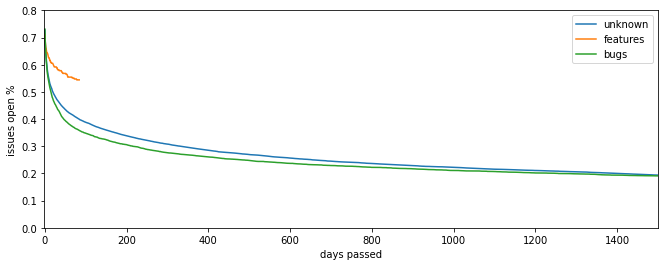
\includegraphics[width=0.9\textwidth]{figures/issues_open.png}
    \caption{Survival curves of the \texttt{pandas} library.}
    \label{fig:survival}
\end{figure}

The last measure is \textit{bug or feature}. Because issues can cover a wide range of possible topics, from discussions to performance, it is worth categorizing them to analyse the differences. However, categorization in practice proves to be difficult due to the different conventions each project uses, and because GitHub does not apply any constraints to the text of the title. We are searching for specific keywords in the \textit{issue title} to categorize each issue into either a bug or a feature. We also drop some of the words from the text, because they would give us 'false positive' matches. If keywords for both or neither categories are found, the issue is marked as unknown. The dropped words, as well as the bug and feature keywords can be seen in Table \ref{tab:keywords} Although this simple method can already classify 10-15 percent of issues, it would require extensive manual effort to further improve this ratio. In future research, sentiment analysis of issue titles and issue descriptions could achieve much higher percentages.

Statistics for issues like average close time also prove to be difficult, because there are continuously open issues, which inevitably leads to the fact that a large portion of issues were still open and continue to be open. For these issues, we cannot know the issue close time, and if we try to calculate global measures by aggregating all (or portion) of issues, we have to consider the \textit{survival bias} \cite{jarczykSurgicalTeamsGitHub2018}. Figure \ref{fig:survival} shows the issues survival curve of the \texttt{pandas} library. It is clearly visible, that a large portion (20 percent) of issues are not closed, and if we left them out of aggregate values such as average open time, our data will be skewed. Nevertheless, we can see in the example, that the categorization of issues makes a difference, as bugs get closed a bit earlier than an average (unknown) issue, because after the same amount of days passign for both categories, more bugs tend to be closed in this example. In contrast, features have a high life expectancy, as they are more likely to be still open than a bug, if the same number of days pass. The reason could be that features take longer to develop and plan than bugs, which is consistent with the findings of Jarczky et. al. \cite{jarczykSurgicalTeamsGitHub2018}.

\begin{table}
    \centering
        \begin{tabular}{| c | c | c |}
            \hline
            \textbf{Drop words} & \textbf{Bug keywords} & \textbf{Feature keywords} \\
            \hline \hline
            debug & bug & feature \\
            debugger & defect & enhancement \\
            debugging & incorrect & improvement \\
             & unexpected & suggestion \\
             & error & wishlist \\
             & missing & wish list \\
             & warning & \\
             & problem & \\
            \hline
        \end{tabular}
    \caption{Keywords and drop words for \textit{bug} and \textit{feature} categorization.}
    \label{tab:keywords}
\end{table}


\section{Collaboration pattern analysis}
\label{sec:patterns}
The focus of our analysis is how the collaboration network of FLOSS projects changes during their lifecycle. Moreover, we are also interested in the cause of the changes, rather than just observing the changes. Therefore we determined two types of events, that we want to observe in order to see the effects on the collaboration. The events during a project's lifecycle can be one of two types: regular or irregular event. Regular events repeat over time with roughly the same time passing between events. This can be a holiday season (e.g. summer holidays or at the end of the year) or regular software releases. In our research, we will focus on only the software releases, and we suggest the analysis of collaboration and seasonality as a future research topic. In contrast to releases, which are usually well documented and easily discoverable when exactly they were released, irregular events are harder to discover, as these do not necessarily stem from within the developer community, but from external sources. Examples could be a supporting company's organizational restructuring, the sudden increase of work from home during the COVID pandemic, or mass layoffs within the support team. In our analysis, we will mainly focus on layoff events, because of our expectation that this will have the largest effect on collaboration. Usually when a company develops an open-source software, the company relies on the external community of the project, but the core developers are mainly from the company. Therefore, when a company officially pulls out from further development, this results in the removal of most core developers in a short amount of time. Our main goal is to identify how this affects the collaboration network, how the network restructures itself, or if any restructuring occurs at all.

As a first step, we conduct a qualitative analysis on a number of hand-picked repositories to observe the network statistics in detail and to identify cause and effect relationships. In order to avoid bias when selecting repositories, we choose projects based on a variety of factors:

\begin{itemize}
    \item \textit{Project size:} We define the project's size as small, if it has less than 100 contributors, medium sized if the number of collaborators are between 100 and 500, and large if it has more than 500 collaborators.
    \item \textit{Centralization:} Although it is hard ot measure how decentralized a project is, based on the literature review, very large projects tend to be decentralized. For now, we consider those projects centralized, which have been identified as centralized in the current state-of-the-art literature. 
    \item \textit{Event occurrences:} Whether there is a regular release cycle within the project or not based on the release dates, or if there are known and confirmed cases of unexpected layoff events.
\end{itemize}

Based on these criteria, we try to select a wide variety of projects, so that each type (small, medium or large size, centralized or decentralized, regular or irregular or abandoned projects) has at least one example. We acknowledge the fact that this inclusion criteria leaves room for selection bias, as an observed correlation between events and the network in one project might not hold true for all projects. However, later we confirm our hypotheses with a quantitative analysis.

\subsection{Project selection and descriptions}

All together we choose 8 projects to analyse, these can be seen in Table \ref{tab:projects}. Due to the repository miner's limitation, we are only considering projects maintained on GitHub. The \texttt{pandas} and \texttt{numpy} repositories are well-known and popular data science tools for data manipulation in Python. They are very similar in size and popularity, both with a huge base of collaborators. Since also the number of issues are really high, our expectation is that these projects are highly decentralized, where the developers mainly work on their own parts of the project. They also have fairly regular release cycles, with a minor release in every 5-6 months.

\texttt{Networkx} and \texttt{seaborn} are both middle-sized repositories based on the number of contributors, and they are both used for data visualization and statistical analysis in Python-based software, but \texttt{networkx} visualizes networks and their related statistics, while \texttt{seaborn} creates various plot images. Each release date follows the previous with 4 to 10 months, which means their releases are not as regular as the first two repositories.

The project \texttt{curl} is an example for a highly centralized project, as its source code is famously maintained by a single developer \cite{crowstonHierarchyCentralizationFree2006}. Based on the number of contributors, it is a medium-sized project, although the number of commits are much higher than \texttt{networkx} or \texttt{seaborn}. Being the oldest project from the selection might contribute to the large number of commits.

\begin{table}
    \centering
    \resizebox{0.85\textwidth}{!}{%
        \begin{tabular}{| c | c | c | c | c | c | c |}
            \hline
            \textbf{Name} & \textbf{Contributors} & \textbf{Size} & \textbf{Commits} & \textbf{Stars} & \textbf{Issues} & \textbf{First release}\\
            \hline \hline
            pandas & 2333 & large & 26792 & 29700 & 3518 & Feb 20, 2011 \\
            numpy & 1135 & large & 26392 & 17200 & 2030 & Jan 5, 2002 \\
            networkx & 469 & medium & 6470 & 9100 & 166 & Jul 17, 2005 \\
            seaborn & 140 & medium & 2780 & 8400 & 82 & Oct 28, 2013 \\
            curl & 701 & medium & 27159 & 20600 & 27 & Mar 14, 2000 \\
            servo & 1101 & large & 44084 & 19600 & 3305 & May 22, 2017 \\
            wasmtime & 243 & medium & 8334 & 5200 & 341 & Oct 18, 2016\\
            py-junos-eznc & 69 & small & 2486 & 583 & 76 & Nov 3, 2013\\
            \hline
        \end{tabular}}
        \caption{Collaboration analysis projects and basic statistics.}
        \label{tab:projects}
\end{table}

\texttt{Servo} and \texttt{wasmtime} are both based on the Rust programming language, and they are both used for web applications: \texttt{Servo} is a browser engine, whereas \texttt{wasmtime} is a runtime environment for WebAssembly. Both projects were led by Mozilla and maintained in an open-source environment. The Rust developer team was heavily affected by the Mozilla layoffs on January 15\textsuperscript{th}, 2020 and August 11\textsuperscript{th}, 2020 \cite{lardinoisMozillaLays70,kastrenakesMozillaLaying2502020}, with the second round of layoffs affecting all Rust employees. The \texttt{py-junos-eznc} project is considered small, since it has less than 100 contributors, and it is a Python-based library for automatizing devbices running on Juno OS. On May 27\textsuperscript{th}, 2020, the sponsoring company Juniper Networks laid off its entire open source developers \cite{brasseurFarewellJuniperNetworks2020}. These three projects will be the main focus of analysing unexpected, one-time events and layoffs, where we will take a close look at the network statistics around the mentioned dates.

To reliably compare the projects, we have to consider only a slice of each project, so all of them are compared within the same time period. We take a 3-year period from 2018 to the end of 2020. All projects had their first release before this period, which means this should filter out the initial irregular activities, such as creating directories and restructuring.

\subsection{Commits analysis}

For the selected period, we check the number of commits in each project as a first step. This can be seen on Figure \ref{fig:commits}. To smooth out the stacked area plot, we summed up the number of commits in every 28 days. Purposefully a multiple of 7 was chosen in order to even out the possible irregularities caused by the weekdays and weekends. We can see that all projects are active, with varying magnitude of commits generated each month. The number of commits are consistent with the size of the project, but we can also see that the number of contributors and the number of commits are not completely dependend on eachother, as \texttt{servo} consistently receives more commits than the other large repositories, despite the fact that it has the same number of contributors as \texttt{numpy} and half as many as \texttt{pandas}. Our assumption is, that this is highly dependent on the type of software being developed, the used programming language(s) and on other project-specific properties.

There is a noticeable decrease in the number of commits to \texttt{servo} at the time of the layoffs (August 2020), which signals that the project could have been affected. This cannot be observed for \texttt{wasmtime}. We do not see any evidence of reoccurring trends within the number of commits, e.g. decreased activity during holiday season. There is a reduction in all repositories at the end of 2018, but this is contradicted by a spike in the number of commits at the end of 2019. However, we cannot rule out any periodicity, because this could be hidden due to the 28-day aggregation.

\begin{figure}
    \centering
    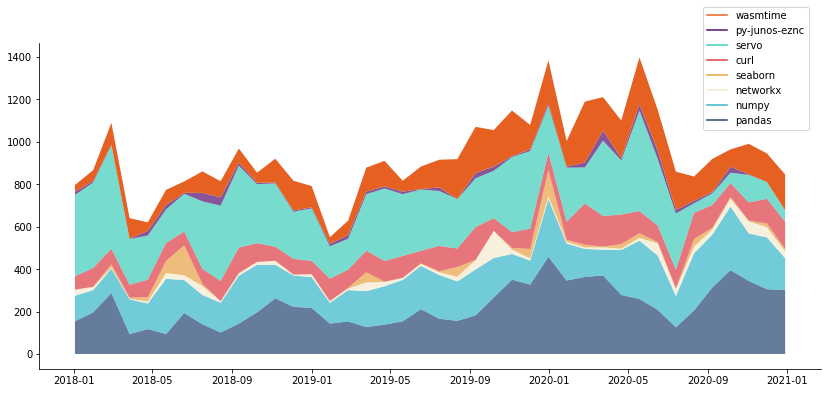
\includegraphics[width=\textwidth]{figures/commits.png}
    \caption{Number of commits in each month.}
    \label{fig:commits}
\end{figure}

\subsection{Releases}
\label{sec:releases}
As a next step, we take a look at the regular lifecycle events, which are the releases in the open source projects. We generate the collaboration networks for the same time period (between 2018 and 2020) and contrast them with the time of releases.

The issue with generating the collaboration network is the time aspect: we cannot observe any collaboration network if we take a single point in time and create the network for a given timestamp, as this will only contain a handful of connections, who authored an edit in the same file at the exact same time. Therefore, we need to aggregate the edits and commits over time, which requires us to use a time window to scan through the observed time period, and for each step, we generate a snapshot of the network. The first parameter is the time window length and the second is the step size. By choosing a large time window, we observe more connetion within the generated graph, but with a too large value, the network becomes too much grouped together, with almost every node connecting to almost all other nodes. By setting this value too low, the result is a disconnected network. The step size determines how often we take a screenshot of the network for the time window. By default, we use one-day steps, but sometimes this results in too radical changes. Therefore in some cases we use a 7-day or a 28-day step value to smooth out the curves. However, a too high step value can obscure the changes we want to observe.

\subsubsection{Node counts}

First we take a look at the number of developers in the network over time. The number of nodes (i.e. developers) in the network indicates the level of activity within the project, where a relatively high number of nodes imply a peak in project activity, and a low number can imply a decreasing activity, or that the project has become more centralised. It is easy to see, that if the only source of activity is one single developer over the observed period, then the network will only have one node, whereas if the same activities are distributed, more developers will be shown in the network, and the number of nodes will rise. However, this does not describe the relationship between developers, they could be completely isolated, or they could be relying a lot on eachother regarding collaboration.

\begin{figure}
    \centering
    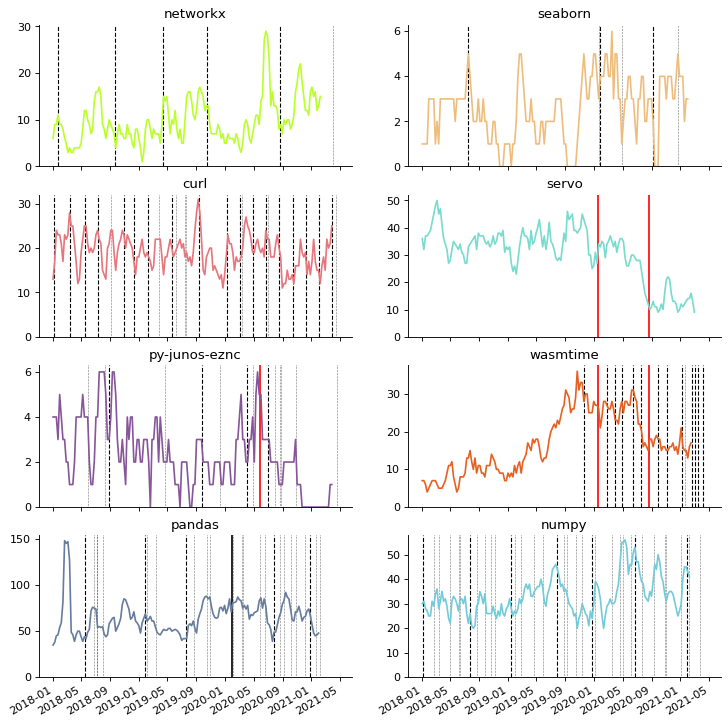
\includegraphics[width=\textwidth]{figures/qualitative/number_of_nodes/all.png}
    \caption{Number of nodes over time.}
    \label{fig:nnodes}
\end{figure}

In Figure \ref{fig:nnodes} the number of nodes are plotted with the time of releases marked with a vertical black line for each project. The type of release corresponds to the type of line: major releases are shown with a continuous line, minor releases are thick dashed lines, and patch releases are thin dotted lines. The red continuous lines mark an unexpected layoff event, which might had an effect on the project. Each node count data point at $t$ time represents the number of nodes within the collaboration network that is generated between $t$ and $t+28$ days, with a 7-day step size. The average node counts correlate with the size of the project, as the smaller repositories like \texttt{py-junos-eznc} and \texttt{seaborn} have the number of nodes consistently below 10, while the larger projects can reach 30, 50 or even 100 at certain time periods.

Regarding the releases, we can see that each project can have completely different release planning and schedule, which makes it hard to compare them. Some projects, like \texttt{networkx}, \texttt{pandas} or \texttt{numpy} release a minor version in approximately every 6 months, while \texttt{curl} does the same in every 2 months. \texttt{wasmtime}'s release schedule regaring minor releases is even shorter, but we do not have any data available before 2020, which does not allow us to confirm whether this is a long-term trend. The release data for \texttt{servo} was available to us, however, the repository has a very high frequency of releases, with sometimes multiple minor releases in the same week, and displaying this information on the chart would have obscured the number of nodes plot, therefore we only display the unexpected events. Also, releases can be arbitrarily named by the developers, therefore a minor release in one project might be considered a patch or a major release in others.

Comparing the events with the number of nodes, we can observe, that before or around a minor release, most projects experience an uptick in node count, which is then usually followed by a drop - although not in every case. This can be contributed to the increased activity from the community before the release. There could be a number of factors that cause this activity change: first, if the release date is fixed, the pressure on developers to include the planned features increases, which prompts more activity (pull model). Secondly, the rise in activity could be a newly implemented feature or a recently found bug, which needs immediate attention from developers. In this case it is possible, that the increased activity and larger volume of edits prompts a new release version (push model). Our assumption regarding whether a release follows a push or a pull model is that it can be highly dependent on the project, and within each project there could be a mixture of releases following both models. We cannot observe this trend for the patch releases, and we cannot draw a definitive conclusin regarding major releases, as there was only one major release among all the repositories subject to our analysis.

Regarding the layoff events marked with red vertical lines, a significan drop in the number of nodes can be observed shortly before the event in all projects. After the companies stop supporting the project and lay off the development team or they are reassigned to other topics, the number of nodes within the projects drop and stay low, never reaching the same numbers as before. In case of \texttt{servo} and \texttt{wasmtime}, the first wave of layoffs do not seem to have a significant impact on the number of nodes, however, we do not have reliable information regarding how much the Rust development team was impacted by the first wave, on which both projects depend.

\subsubsection{Network density and mean degree}
As a next step, we plot the network density and mean degrees of the projects. The network density tells us how densely connected is the network in a scale of $[0,1]$, where 1 means every node is connected to all other nodes, and 0 means there are no edges in the graph. It refers to the ratio between all the possible connections and the actual connections. Although the generated networks are weighted, we do not consider the edge weight when counting each node's degree, meaning every connection is counted. We expect this value to rise if developers need to reach out to more members of the community and collaborate on more files with others. Similarly to the density, the mean degree value also only takes the number of nodes (N) and the degree number (k) of each node as inputs, so we expect similar results between the two measures.

By plotting the two measures on the same figure in Figure \ref{fig:density_a}, we can confirm, that they are closely correlated. The values are also highly sensitive regarding the number of nudes within the graph, and a low node count makes the graph values change radically. This is why the smaller projects are not shown, as their graph did not convey any meaningful observations. We can identify some troughs at the release times of minor releases, however, these could also be the results of the changes in the number of nodes.

\begin{figure}
    \centering
    \begin{subfigure}{0.53\textwidth}
        \centering
        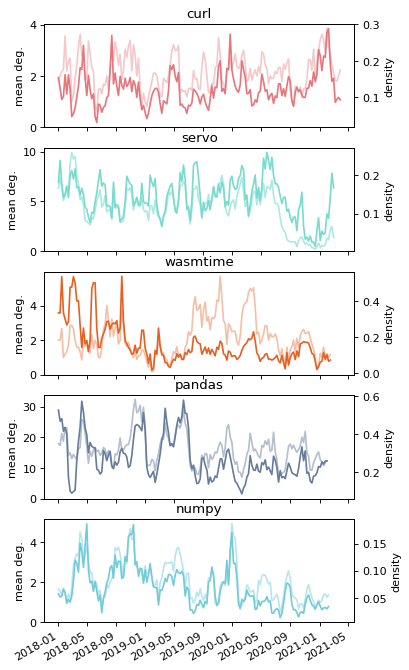
\includegraphics[width=\textwidth]{figures/qualitative/mean_deg_density/mean_deg.png}
        \caption{Density (dark) and mean degree (light).}
        \label{fig:density_a}
    \end{subfigure}
    \begin{subfigure}{0.46\textwidth}
        \centering
        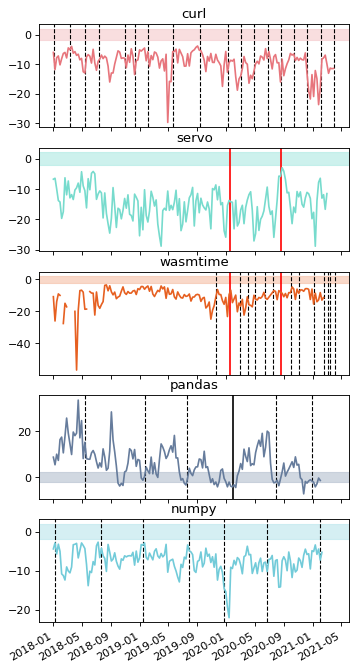
\includegraphics[width=\textwidth]{figures/qualitative/mean_deg_density/mean_deg_z_values.png}
        \caption{Z-values for density and releases.}
        \label{fig:density_b}
    \end{subfigure}
    \caption{Network density, mean degree and Z-values over time with significance threshold highlighted.}
    \label{fig:density}
\end{figure}

In order to adjust the network statistics for their sizes, we compare the network with a randomly generated, same-sized network. If we see a significant difference between the two values, we can confidently state that the changes we observe in the network statistics are independent from the network size. To measure the significance, we calculate the \textit{Z-value} of the actual network statistic and a 'general' network of the same size. In our implementation, we randomly generate 10 networks with the same number of edges and nodes as the original network, and use them to calculate the Z-value. The Z-value's formula is:

\[ Z=\frac{x-\mu}{\sigma} \]

where $x$ is the actual value we are comparing (in this case the network density), $\mu$ is the average network density of the randomly generated networks, and $\sigma$ is the standard deviation of the random graphs. We consider a network significantly different than a random network if its Z-value is greater than $2$ in absolute terms. When the Z-value of network density is lower than $-2$, the network has a lower density than a same-sized general network, meaning the edges are more dispersed. Similarly, a Z-value greater than $2$ signals that the graph has more central hubs than the random network.

We plot the Z-values over time in Figure \ref{fig:density_b}, where the area between $-2$ and $2$ are colored to show at which times the network is significantly different than a randomly generated one: when the plot line is within this range, it is not significantly different, otherwise it is. In some cases, there is a break of continuity within the plot. This occurs, when the standard deviation of the randomly generated network is $0$, which would result in a zero-division error. The standard deviation can only be $0$ when all the values are the same, which means in these cases our randomly generated networks have exactly the same density. This usually happens in extreme cases, when there is a very low number of nodes or edges.
  
Almost all projects have a significantly low network density, meaning that the edges are more distributed between the nodes. The notable exception is the \texttt{pandas} repository, which has an overall positive Z-value over time, with sometimes crossing the insignificant zone. These points are mostly troughs at the time of minor releases. We can also see on all projects, that around a release, the Z-value approaches (or crosses) the threshold, which signals that the networks behave more like random networks around releases. The same can be observed for the layoff events, as \texttt{servo} gets really close to $-2$ at the time of the announcement.

\subsubsection{Clustering coefficient}

The weighted global clustering coefficients explained in Section \ref{sec:clustering} is plotted over time in Figure \ref{fig:clust}. Because it would be difficult to show both the Z-values and the the clustering coefficients on the same graph for each project, we change the color of the line to indicate the statistical significance. Where the clustering coefficient is significantly different from a random network to the negative side (meaning the Z-value at the corresponding date is less than $-2$) the line uses the project's dark shaded color. Likewise, when there is a significant difference and the Z-value is over $2$, the dark complementer color is used. Within the range of $[-2, 2]$ a light color is used to signal the statistical indifference from a random network of the same size. The color label also indicates the associated Z-value within each subgraph.

\begin{figure}
    \centering
    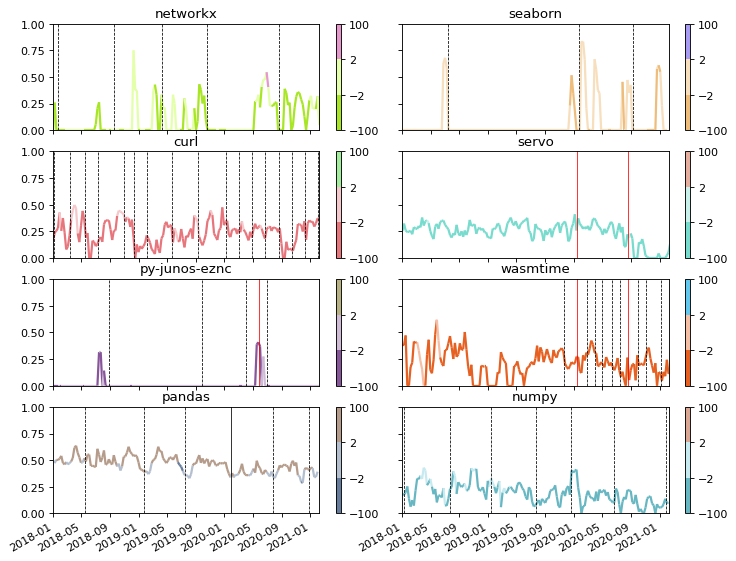
\includegraphics[width=\textwidth]{figures/qualitative/clustering_coeff/clustering.png}
    \caption{Clustering coefficients over time.}
    \label{fig:clust}
\end{figure}

We receive mixed results for the clustering coefficients. The smaller libraries (\texttt{networkx}, \texttt{seaborn} and \texttt{curl}) show a sudden spike before a release, which means that the network gets clustered before a release. However, the Z-value is always showing a negative sign being less than $-2$ in these cases (with the notable exception of \texttt{pandas}, which is mainly above $2$), signaling that the increase in clustering coefficient is significanly less than a same-sized random network. This shows, that the spike and then a drop in the clustering coefficient before a release is caused by a sudden increase and then decrease of activity within the project, but this activity is decentralized and affects all developers roughly the same. One of the reasons is the more decentralized workflow: as Crowston et. al. \cite{crowstonHierarchyCentralizationFree2006} have identified, smaller projects early in their lifecycles tend to be more centralized, as there is less specialization to only one area of the project.

Interestingly, almost all of the larger projects have consistently lower clustering coefficient than of a random network, which indicates, that there is a significant overlap of the edited files within the projects, and there is less specialization. Another explanation could also be the use of shared files, which relates to the project structure. If an implementation of a new feature requires developers to edit almost all existing files by adding new functions, then the clustering coefficient will be low. On the other hand, if every new feature requires a new file to be added, developers will be mostly isoated in the collaboration network around the files, which will show up as a higher clustering coefficient than in a random network. This would explain why the \texttt{pandas} library has consistently a positive Z-value: the project structure does not require contributors to edit eachother's files. Additionally, we can observe a drop in the clustering around releases, but without statistical significance. This also confirms, that the network becomes more random-like around releases, but we can further extrapolate that a likely factor to this phenomenon is the feature integration: between releases, contributors center around their specialization editing only a limited number of isolated files, but before the release, the effort shifts towards integrating these features together, which requires editing files outside of the 'usual folder'.

\subsubsection{Mean path length}

Another measure that could be affected by a releaase is the length between nodes in the network. From an organizational perspective, a path between two contributors represent the information flow regarding a specific part of the project. If in a network every vertex tends to be close to the other nodes, meaning less jumps are required, then they are able to gather information about a specific part of the project quicker. Smaller projects with less contributors naturally have relativel short connections to all other developers, and as the software gets larger with more contributors, the average shortest path between nodes is expected to get longer. However, if the project structure maintains central connecting 'hubs' (in this case: developers), the growth in length can remain lower.

In an undirected unweighted graph, the shortest path between two nodes is the least amount of edges needed to be touched in order to get from one node to the other. However, our collaboration network is a weighted undirected graph, where the edge weights represent the collaboration effort between two developers. A strong collaboration is represented as a higher edge weight, whereas a lower edge weight means there is less collaboration between the two contributors. The shortest path between two nodes in a weighted graph is the path, which has the least summed weight of the edges touched. In our case, we want to measure how far away each developer are from all the others in order to quantify the effort for reaching out to eachother in case they want to involve a specific community member. To select the closest connection, we need to look for the strongest connection, meaning we have to consider the longest path between nodes.

\begin{figure}
    \centering
    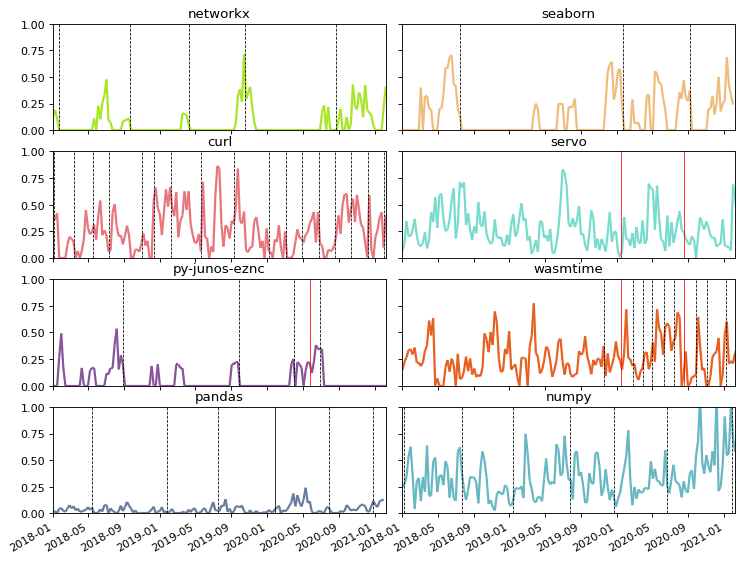
\includegraphics[width=\textwidth]{figures/qualitative/mean_path_length/longest_path_length_all.png}
    \caption{Mean longest path length over time with statistical significance.}
    \label{fig:mean_path}
\end{figure}

We calculate the average longest path $P$ by first summing up all the longest paths from a given node to all other nodes, then dividing by the number of connections, which is $n-1$ in a connected graph. Then we sum up all of these averages for all nodes, and divide by the number of nodes $n$:

\[ P = \frac{\sum{_{i=1}^{n}} \sum{_{j=1}^{n} -w_{ij}+1} }{n(n-1)} \]

where $w_{ij}$ is the edge weight between $a_i$ and $a_j$ in range $[0, 1]$. We multiply the weights by $-1$ and add $1$ in order to calculate for the longest, and not the shortest path. If there is no edge between $a_i$ and $a_j$, then $w_{ij}=0$.

It is clearly visible in the smaller projects (\texttt{networkx}, \texttt{py-junos-eznc}, \texttt{seaborn}), that the path length increases before a release due to the increased activity, and otherwise it stays $0$. This indicates a 'push-type' release process, where the releases are sporadic, and a new release is created to incorporate and deploy the changes implemented. With the other projects, we do not see any correlation between releases and mean path length.

\subsubsection{Core and periphery analysis}

Around releases it is reasonably expected that the ratio between core and periphery developers changes. It has already been established, that within a project, the core members tend to stay the same throughout the project's lifecycle, but the tasks regarding the new release preparation might change their relation with the periphery community members. The first method we use to identify core members is explained in Section \ref{sec:deg_centrality}. We call the number of core members identified this way as \textit{Degree centrality core} value. 

Besides taking the 20th percentile of the top clustering coefficients to identify the number of core developers in the network, we also use the degree number of each developer to identify their \textit{K-core value}. The K-core of a network is the subset of nodes, which have at least $k$ degrees, and we call the network's K-core value the number of nodes within the K-core \cite{batageljAlgorithmCoresDecomposition2003}. Then, we identify the vertices, which are in the top 20th percentile of K-cores, as core developers. For example, if the maximum number of degrees within the network is 10, then the K-core value is the number of nodes, which have at least a degree number of 8.

We observe the ratio between the number of core and periphery developers by dividing the number of core developers with the number of nodes within the network. This gives us a ratio between $0$ and $1$ for both the \textit{Degree centrality core} and the \textit{K-core value} methods, where $1$ means the network only contains core developers. It is important to note that the only case both methods can have $0$ as a core/periphery ratio is when there is no collaboration within the network and all nodes are isolated with a degree of $0$. We then plot the Z-values for both methods' core/developer ratio as before, which can be seen in Figure \ref{fig:core-periphery}.

\begin{figure}
    \centering
    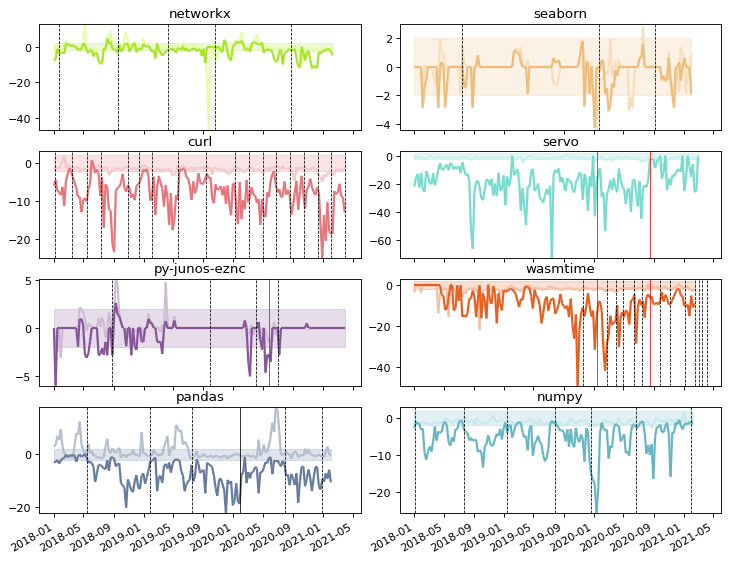
\includegraphics[width=\textwidth]{figures/qualitative/core_periphery/core_periphery_all.png}
    \caption{Core/periphery ratio's Z-value over time with K-core and Degree centrality methods.}
    \label{fig:core-periphery}

\end{figure}

The lighter colored plot line shows the Z-vale over time for the core and periphery ratio based on the Degree centrality method, whereas the darker line shows the same ratio calculated with the K-core method. We can see again a sharp difference between the smaller and larger projects. For the smaller projects, the two measures roughly behave the same, as their plots overlap for most of the time. Most of the time these values stay within the statistically insignificant range and only in these cases are significantly different than a random network.

In contrast, the large projects have their K-core ratios consistently below $-2$, indicating that the core ratio is consistently lower than a randomly generated network, which signals its centralized property. This cannot be said for the Degree centrality core ratios, which are consistently within the insignificant range. Just as with the smaller projects like \texttt{networkx}, \texttt{seaborn} and \texttt{py-junos-eznc}, we can observe a significant drop in K-core ratio Z-values within 2 to 3 months after the release. The difference between the two networks are demonstrated for \texttt{numpy}'s minor release on 22.12.2019, where the networks for 1-month after, and 1-month before are contrasted in Figure \ref{fig:core-periphery-numpy}.

We can see the nodes identified as core highlighted with blue. In Figure \ref{fig:numpy-before}, we can see that the maximum number of degree is paired with a couple of similarly connected nodes, and this is combined with a relatively small number of nodes in the graph, which results in a relatively high number of core members with a low number of periphery, therefore the ratio gets higher, which is more similar to an almost completely dispersed random network. Whereas in Figure \ref{fig:numpy-after}, we can observe the opposite: the small number of core member (only one) is combined with a large number of nodes, which creates a low core-periphery ratio, that is significanly lower than in a randomly generated same-sized network. The fact that the second graph has more nodes and they are more connected lets us draw the conclusion that the increase in activity is the effect of the release, where after the new version release to the public led to an increase in bug reports, which caused a surge in activity as they are being fixed.

\begin{figure}
    \centering
    \begin{subfigure}{0.49\textwidth}
        \centering
        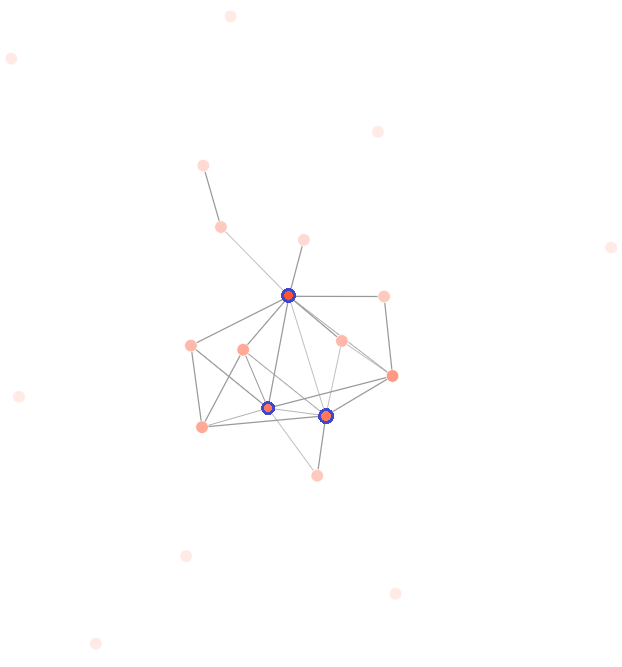
\includegraphics[width=\textwidth]{figures/qualitative/core_periphery/numpy_before.png}
        \caption{Between 2019-12-09 and 2020-01-06}
        \label{fig:numpy-before}
    \end{subfigure}
    \hfill
    \begin{subfigure}{0.49\textwidth}
        \centering
        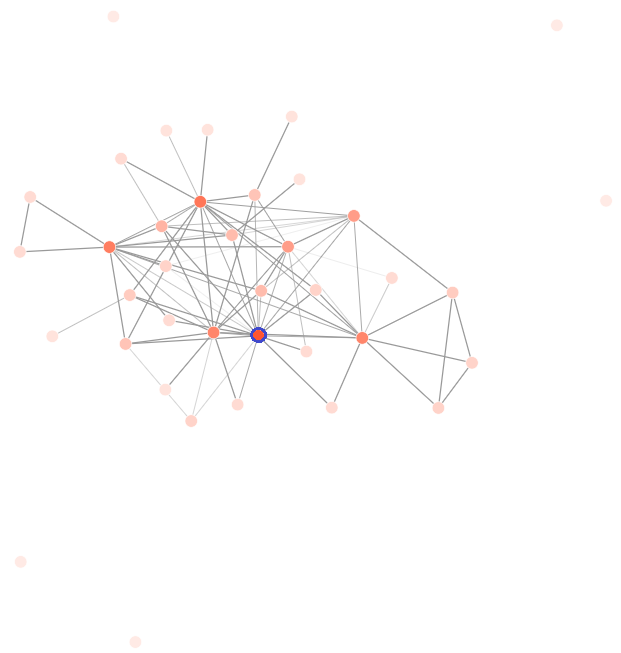
\includegraphics[width=\textwidth]{figures/qualitative/core_periphery/numpy_after.png}
        \caption{Between 2020-01-06 and 2020-02-03}
        \label{fig:numpy-after}
    \end{subfigure}
    \caption{\texttt{Numpy} collaboration network before and after the 2020-12-22 minor release.}
    \label{fig:core-periphery-numpy}
\end{figure}

The notable exception for the K-core values in Figure \ref{fig:core-periphery} is again \texttt{pandas}, where the Degree centrality core-periphery ratio determines each release nicely: we can consistently see a positive spike above the significance level 2 months before each release. This finidng is consistent with the degree centrality analysis, however, here it is more pronounced. The drop after the release in K-core ratio also seems to hold true.

In general we can say that especially in larger projects the core can be clearly separated from the periphery developers, as the Z-values show significantly lower values than of a random network regarding the core/periphery ratio. We can also observe in projects with more contributors, that a release causes the Z-values to rise, which indicates that the graph becomes more even. We can conclude from this observation, that more periphery contributors are active around a release, confirming the theory that an upcoming release triggers more activity as developers want to push their changes to the upcoming release.

\subsubsection{Hierarchy}

As a last step, we take a look at the hierarchy of the networks over time. We use the method described in Section \ref{sec:hierarchy} and we plot the linear regression's $\beta_1$ value (the slope of the trendline). Figure \ref{fig:hierarchy_all} shows these values over time per observed project, where the darker line color indicates a significant Z-value in either direction (less than $-2$ or larger than $2$).

\begin{figure}
    \centering
    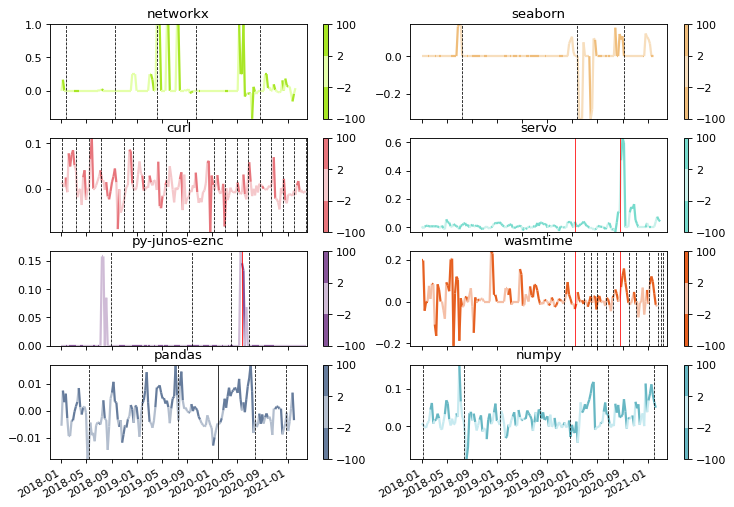
\includegraphics[width=\textwidth]{figures/qualitative/hierarchy/hierarchy_all.png}
    \caption{Hierarchy over time}
    \label{fig:hierarchy_all}
\end{figure}

In \texttt{networkx} and \texttt{seaborn} we can see activity only around releases, which is due to the fact that there aren't enough commits and developer activity to properly form a collaboration network, so it defaults to zero. Therefore, we can contribute the hiererchy change in their cases to the change in network size.

Just as with the other statistics, \texttt{curl} has a frequent and regular release plan, which makes it hard to observe any regularities around releases. We can see some spikes and some troughs coincidentally at the same time as the releases, but there isn't any consistency between them, and therefore we cannot conclude a definitive cause and effect between hierarchy and releases. Unlike the other projects, \texttt{curl} has a lower hierarchy score as it frops below $0$ many times, indicating a somewhat more hierarchial structure. This is expected, as it is known that it is mainly developed by a single developer, which results in high hierarchy.

In case of \texttt{servo}, \texttt{py-junos-eznc} and \texttt{wasmtime} the hierarchy seems to correlate with the unexpected events closely. In \texttt{servo} there is a definitive spike exactly at the second layoff event, which clearly indicates a huge change in the network. It has a large nubmer of contributors, which results in a comparatively smooth curve within the other projects, as it rarely goes above $0.1$ and it is always above $0$. Similarly, \texttt{py-junos-eznc} also shows the only significant Z-value at the time of the layoff event with a positive spike. \texttt{wasmtime} also shows the largest positive spike within a 2-year period at the exact time of the layoff, which leads us to conclude that the sudden decline of hierarchy (it is more hierarchial if the value is negative) is a good indicator of the layoff events. This can be explained by the removal of core contributors, as the teams are disrupted and developers have to collaborate directly with more of their peers, as opposed to going through the established channels.

\subsection{Release regularity}
\label{sec:release_reg}

During the network measure analysis we recognized that the regularity of the releases can have a great effect on how it changes the network. In smaller projects a push-model can be recognised, where the new features are added, and then a new release is created, which incorporates this feature. This ensures that the new feature gets deployed as fast as possible. In these cases we can see that the releases do not happen regularly, but when there is a release, there is a significant change before or after it.

Projects that follow a pull-model tend to have more regular release periods, and they are also the large projects in our analysis. Within these projects the flow of new features and bug fixes are constant, and they are deployed within a fixed period of time. Therefore, the new release does not necessarily have a visible impact on the network, because if the feature is not complete yet, it will be released in the next one. A great example for this is the \textit{1.0} release of \texttt{pandas}, which does not show any more network change in any metrics compared to a minor release despite being the only major release within all eight projects - contrary to the expectations.

In order to quantify the regularity of the releases within the project, we calculate the \textit{coefficient of variation} (CV) within each project for the days between each release. The $CV_i$ is the ratio of the standard deviation $\sigma$ to the mean $\mu$ of number of days passed between two releases for project $i$, which can also be interpreted as a percentage \cite{everittCambridgeDictionaryStatistics1998a}:

\[ CV_i = \frac{\sigma_i}{\mu_i} \]

It must be determined for each type of release, because we have seen, that the type can have an effect of regularity. For example, in some projects patches follow up on a minor or major release, which can make the overall releases irregular, even though major and minor releases could still follow a regular pattern. We measure the release regularity CV in Table \ref{tab:regularity}. In order to calculate the value, the project must have at least two releases per type to have at least one value for days passed between releases. In cases when this condition is not met, we leave the values empty.

\begin{table}
    \centering
    \resizebox{\textwidth}{!}{%
        \begin{tabular}{| l | c | c | c | c | c | c | c | c |}
            \hline
            \multirow{2}{7.5em}{\textbf{Project name}} & \multicolumn{4}{|c|}{\textbf{Minor+Major releases}} & \multicolumn{4}{|c|}{\textbf{Patch releases}} \\
            \cline{2-9}
            & \textbf{$N$} & \textbf{$\sigma$} & \textbf{$\mu$} & \textbf{$CV$} & \textbf{$N$} & \textbf{$\sigma$} & \textbf{$\mu$} & \textbf{$CV$} \\
            \hline
            \texttt{pandas} & 6 & 34.93 & 191.2 &\textbf{0.1827} & 21 & 47.72 & 48.15 & \textbf{0.9911} \\
            \texttt{numpy} & 7 & 22.91 & 186.67 & \textbf{0.1227} & 29 & 22.44 & 40.39 & \textbf{0.5554} \\
            \texttt{networkx} & 5 & 46.70 & 235.75 & \textbf{0.1981} & 1 & - & - & \textbf{-} \\
            \texttt{seaborn} & 3 & 164.5 & 392.5 & \textbf{0.4191} & 3 & 71.5 & 166.5 & \textbf{0.4294} \\
            \texttt{curl} & 18 & 24.19 & 69.53 & \textbf{0.3479} & 8 & 99.29 & 136.0 & \textbf{0.7301} \\
            \texttt{servo} & 116 & 8.31 & 8.67 & \textbf{0.9585} & 189 & 4.99 & 5.05 & \textbf{0.9876} \\
            \texttt{wasmtime} & 13 & 24.49 & 41.91 & \textbf{0.5843} & 1 & - & - & \textbf{-} \\
            \texttt{py-junos-eznc} & 4 & 127.68 & 224.33 & \textbf{0.5692} & 10 & 84.51 & 117.44 & \textbf{0.7196} \\
            \hline
        \end{tabular}
    }
    \caption{Release regularities for major, minor and patch releases.}
    \label{tab:regularity}
\end{table}

The coefficient of variation has a lower bound of $0$ in our case, because the number of days passed between two release can never be a negative number - the smallest possible is $0$ when the release dates are exactly the same days apart from eachother. However, the CV has no upper bound, as the standard deviation can be arbitrarily large, and larger than the mean release days. Also, there is no unit associated with it, so we can only give meaning to the CV value in the context of other projects as comparison: a project with a smaller CV value has a more regular deployment schedule than another one with a higher CV. Since its scale is a ratio scale, we can also interpret a two times larger value as "two times more regular interval".

We also note that although the coefficient compensates for the difference between mean values, it does not take into consideration the number of intervals observed. This means that a one-day delay of a release from an established schedule does not have a large impact when there are 100 other releases, which are on time, but if there are only 4 releases, this changes the mean significantly and therefore the CV too. This is why we also display the number of releases as $N$. \\

It can be observed in all projects, that the minor and major releases are more regular than the patch releases. This confirms the theory that patch releases are mainly added as bug fixes for minor and major releases after they are made public, and they do not folow a regular pattern. The difference between patches and major-minors are not consistent within the repositories: the greatest difference is in \texttt{pandas}, where the patch CV is five times larger than the minor-major CV. Close second is \texttt{numpy} with a similar 4.6 times larger irregularity of patches. Both projects have roughly a 180-day release cycle, and it is clearly visible that patches directly follow the minor releases in Figure \ref{fig:nnodes}, and they get sparser as we get further away from the minor releases in time.

The repositories \texttt{networkx} and \texttt{wasmtime} do not have enough patches within the observed period to calculate the patch values, therefore we cannot compare them to the major-minor releases. The \texttt{networkx} repo has a much more regular minor release cycle than \texttt{py-juno-eznc}, which has a similarly large release cycle of about 230 days. This indicates that small-sized projects, which usually have longer release cycles, can also vary a lot depending on the project, and they can be just as regular as a larger repository. \texttt{Seaborn} is somewhere in between the previous two in terms of regularity, however, with only 3 minor and 3 patch releases, we cannot say any definite about comparing it to other projects, because we cannot say for sure that the middle release of the 3 is an outlier of the many regular releases, or it is completely random even if we go back further in time to check a larger number of releases.

\texttt{Curl} has one of the shortest minor release cycles with an average of 70 days, and it is regular with a CV of $0.35$, which confirms what we have observed visually on Figure \ref{fig:nnodes}. A short but regular release cycle will result in more added releases over a fixed time period, which leaves room for more errors. Furthermore, with a short release cycle only a small delay is required to have a great impact on the CV value. Therefore we believe that this method could be biased towards small release cycles, and they are shown as less regular than a larger, 180-day cycle shows. Nevertheless, it is still clear from the coefficient, that \texttt{curl} is one of the regular projects.

\texttt{Servo} has an extremely short release plan with only an average of 8-9 days between minor releases. We can also see the bias against shorter cycles, as it has by far the largest coefficient of variation with $0.96$. Due to the short time between releases, it is enough to delay a release by just a couple of days to significantly worsen the CV score. However, with a standard deviation also being around 8, we can see that the regularity cannot be as precise as in \texttt{pandas} or \texttt{numpy}, despite the bias. \\

Considering the plotted graphs with the releases, and also the CV values, we want to determine a CV value, that can classify a project into 'regular' or 'irregular' release cycles. We have seen that there is a slight bias against shorter cycles, but finding a way to compensate for it would greatly increase complexity, which could lead to other issues. Therefore, we will use a coefficient of variation of $0.4$ \textbf{for the minor and major releases} to draw the line: every value below that indicates a regular release plan, and everything above that signals an irregular cycle. As stated before, patches tend to folow up on majors and minors, therefore we should not consider them overall.  By this classification, \texttt{pandas}, \texttt{numpy}, \texttt{networkx} and \texttt{curl} are \textit{regular}, whereas \texttt{seaborn}, \texttt{servo}, \texttt{wasmtime} and \texttt{py-junos-eznc} are \textit{irregular} when it comes to release cycles. We can also see visually on the plotted graphs in Section \ref{sec:releases}, that this separation seems to be right.

\subsection{Release efficiency, issues}

So far we have seen how the collaboration network statistics change before, at and after a release. We also categorized the releases based on major, minor and patch releases, where we expected bigger changes in collaboration with a larger release - which was not always the case. Then we categorized the projects into regular and irregular release cycles. As a next step, we want to analyse in this section whether a release is successful or unsuccessful, and how we can measure this success rate.

The common perception of software development is, that a rushed release will have worse quality, which will result in more bugs in the software. This was confirmed by Michlmayr et. al. \cite{michlmayrWhyHowShould2015}, and they name the lack of testing as one of the main source of rushed code. They also identify the two release strategies we mentioned in Section \ref{sec:release_reg}, namely regular, time-based or irregular, feature-based release strategies. They have found, that a feature-based strategy can cause rushed code development and poorly tested features due to the fact that the next release date is unknown. Therefore, contributors are incentivised to submit their changes as soon as possible, so that their changes are deployed to the public users of the open-source software. This unpredictability forces developers to skip or glance over the testing phases, which ultimately leads to more bugs in the software.

A fixed time-based release cycle, on the other hand, is predictable, which allows contributors to plan ahead the tasks related to the new feature or bug fixes \cite{michlmayrWhyHowShould2015}. Furthermore, in case of a delay, it can be already known when the next one will be approximately, and further features can be replanned accordingly. A regular release schedule is therefore a sign of a healthy project, which indicates to the users, that there is active support for the OSS software, and also to developers that the project is set for a longer term, and it is a viable candidate to contribute into.

As a new version is released, the users of the software are notified through the distribution channels, which triggers a spike in downloads due to users wanting to be up-to-date to the latest software version \cite{khomhFasterReleasesImprove2012}. Due to the quick adoption period within FLOSS projects, the majority of bugs are also expected to be reported shortly after a release, with a rushed version possibly having a larger amount of bugs after its release. Therefore, a great measure of release quality can be the number of bugs reported after a release. GitHub's standard bug and feature tracking API is the Issues page, so the number of issues created will be used for this purpose. 

\subsubsection{Issue opening and closing frequencies}

The number of issues opened and closed can be seen on Figure \ref{fig:issues_created_closed}. The issues are sampled in every 14 days, where the 7 days before and after are aggregated, separately for issues closed and issues created. For example, the month January will have two data points: January 8th, which aggregates the period January 1-14, and January 22nd, which will sum up all the number of issues created and closed between January 15-28.

\begin{figure}
    \centering
    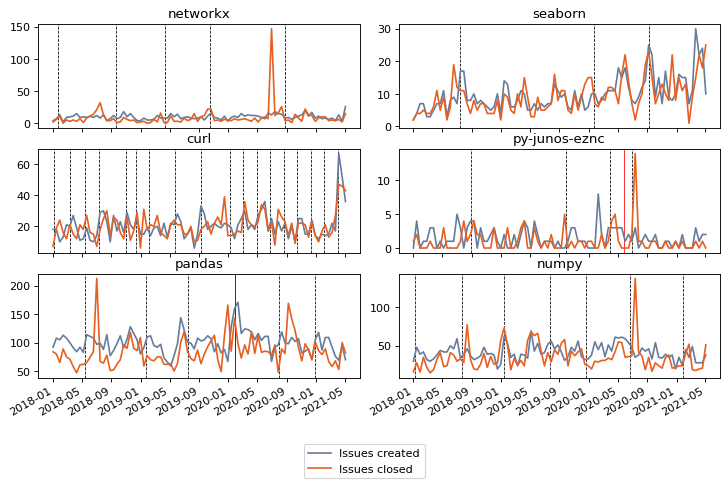
\includegraphics[width=\textwidth]{figures/qualitative/issues_closed_created/issues.png}
    \caption{Issues closed and created per project.}
    \label{fig:issues_created_closed}
\end{figure}

Based on the plots, we can confirm the increased number of issues at a release, as all projects' most release dates coincide with a peak in issues created. Interestingly, the peaks do not necessarily come after or exactly at the release, and sometimes they preceed the actual release date. Some examples are the \texttt{pandas} version \texttt{v0.24.0} on \textit{January 25, 2019} or version \texttt{v0.25.0} on \textit{July 18, 2019}, or \texttt{py-junos-eznc}'s \texttt{2.3.2} on \textit{April 1, 2020}. Most likely this is an effect of successful testing: before the release, the software is thoroughly tested, and all identified bugs are registered as issues. Since most issues are fixed before the release, users do not find more issues than usual, therefore the issues created drops. Similarly, a peak in opened issues after the release might mean a less robust testing system. We can observe this in \texttt{networkx}, where the number of issues created gets higher at the release, or shortly after.

The number of issues closed follows a similar trend. The expectation was, that the issues closed peak before a release, since the planned tasks to be added to the new version are being closed, and after the new release, the issues closed would fall, as most features and bugs have already been implemented in the new version. Although this holds true in some cases, especially in \texttt{networkx} and \texttt{pandas}, this is not the case all the time, as sometimes large spikes occur right after a release, such as \texttt{numpy}'s version \texttt{v1.19.0} on \textit{Jun 20, 2020} or \texttt{pandas}' new release on \textit{May 15, 2018}. Our assumption is, that unusually large spikes like these occur as a 'clean-up' after the release, so the new release cycle can be planned.

\subsubsection{Open issues over time}

Now that we have seen some regularities regarding issue creation and close, we also examine how the number of open issues change with the releases. As we discussed in Section \ref{sec:project_issues}, since there are continuously open issues in an active project, some of which are not closed at the time of taking the project snapshots, we cannot take any averages or aggregation due to the survival bias.

\begin{figure}
    \centering
    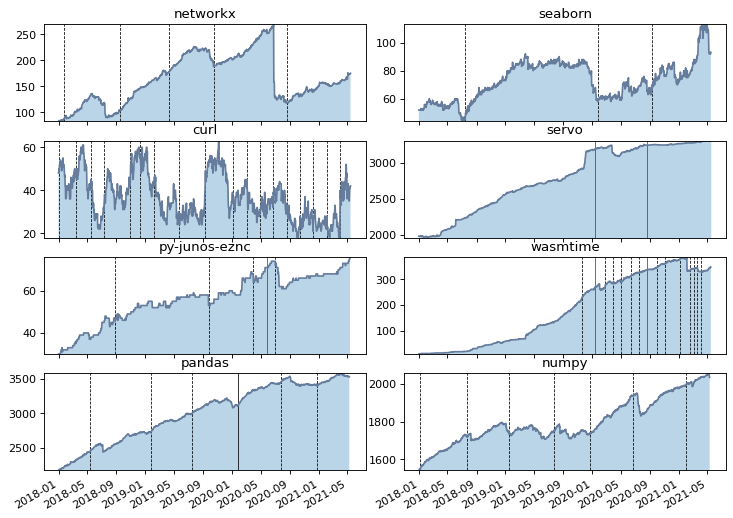
\includegraphics[width=\textwidth]{figures/qualitative/issues_closed_created/open_issues.png}
    \caption{Open issues over time}
    \label{fig:open_issues}
\end{figure}

Figure \ref{fig:open_issues} shows the number of open issues for each project in the observed 3 years. We can see that in almost all projects, the number of open issues steadily rises, with smaller dips occurring around some, but not all releases. This shows, that maintaining and organizing the issues becomes a larger challenge as the project grows, and confirms the large spikes in the number of issues closed on Figure \ref{fig:issues_created_closed}, that these are 'clean-up' events, where the backlog is decluttered by closing the obsolete issues.

The only exception from the ever-growing number of open issues is the \texttt{curl} library, which manages to keep the number of open issues below 60, despite being the oldest project of all 8 subject to our analysis. This could also be related to the short release cycle. As Khomh et. al. \cite{khomhFasterReleasesImprove2012} have found, bugs are fixed significantly faster with rapid release plans. Furthermore, as \texttt{curl} is the most centralized project, with one single main developer, issue management is much more efficient, as there is no need for group discussions and prioritization between developers. Interestingly, \texttt{servo} has the shortest release timing strategy, with sometimes multiple minor releases in a week, yet it is still struggling with the increasing number of issues, indicating that a strongly centralized organizational structure can have a much heavier weight in the increase of open issues over time. \\

\subsubsection{Bugs and features}

Issues can describe many tasks within a project, including ideas, features, discussions, bugs, warnings, depreciation plans, and so on. Each repository organizes the issues with labels, which can be created and color-coded freely within each project. Therefore, the labels cannot be used across projects, as each repository has its own personalised system. For example, \texttt{pandas} uses the tag 'Bug' for bugs, \texttt{numpy} uses '00 - Bug', since they order the labels by giving a number in front of it, and \texttt{servo} doesn't have a bug category, because they divided this category into 'I-crash' and 'I-wrong' among other labels. Also, they categorize the labels by their starting letter, which is not a practice in the other projects.

Seeing which types of issues are affected the most by a release could also provide insight into how the project, and by extension the collaboration network changes. Instead of using the labels, we categorize them with pattern matching in the title as described in Section \ref{sec:project_issues} with the same keywords and method. Even though the matching rate is not expected to be high, we can still apply the method for the projects, because the issues matching a category have a high chance of actually belonging to that category due to the low number of keywords being used, meaning our false positive rate for the classification is presumably low. However, we cannot confirm this, as the manual effort to classify the issues would be too large. The results can be seen in Figure \ref{fig:open_bugs_features}.

\begin{figure}
    \centering
    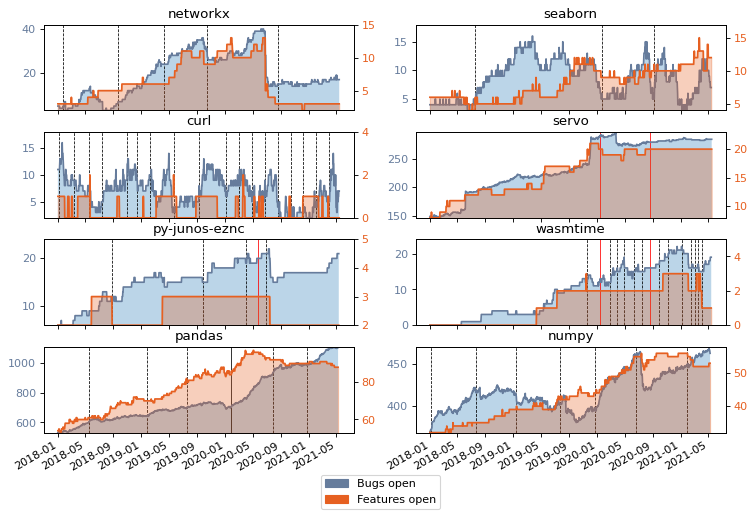
\includegraphics[width=\textwidth]{figures/qualitative/issues_closed_created/features_and_bugs.png}
    \caption{Open bugs and features over time.}
    \label{fig:open_bugs_features}
\end{figure}

The bugs and features are presented on two different scales, because their magnitude is different (there are a lot more bugs identified than features), but we want to compare the relative changes to eachother. Sadly we cannot see any significant difference between the number of bugs and features open, apart from a few exceptions, such as the December 2020 release of \texttt{pandas}, after which the number of open features decline while the number of bugs rise; or the July 2019 version of \texttt{numpy}, where the opposite is true and the features keep rising while the bugs decline.

Since both the features and the bugs curves follow the same shape, which is also the same as the overall shape of the issues, we cannot draw any definitive conclusions regarding the difference between bug and feature issues. The reason for this, is that we are only able to classify a small portion of the issues. When the overall number of issues rise, it makes it more likely to find a feature or bug just by sheer luck, and that is why both curves follow the overall curve. Therefore, we cannot confirm the statement that there is no difference either.

\begin{table}
    \centering
    \resizebox{\textwidth}{!} & N & \textit{\%} & N & \textit{\%} \\
            \hline
            \texttt{pandas} & 20501 & 6245 & \textit{30.46\%} & 294 & \textit{1.43\%} & 13962 & \textit{68.10\%} \\
            \texttt{numpy} & 9536 & 2421 & \textit{25.39\%} & 134 & \textit{1.41\%} & 6981 & \textit{73.21\%} \\
            \texttt{networkx} & 2524 & 384 & \textit{15.21\%} & 54 & \textit{2.14\%} & 2086 & \textit{82.65\%} \\
            \texttt{seaborn} & 1885 & 341 & \textit{18.09\%} & 99 & \textit{5.25\%} & 1445 & \textit{76.66\%} \\
            \texttt{curl} & 2866 & 489 & \textit{17.06\%} & 35 & \textit{1.22\%} & 2342 & \textit{81.72\%} \\
            \texttt{servo} & 11485 & 1016 & \textit{8.85\%} & 57 & \textit{0.50\%} & 10412 & \textit{90.66\%} \\
            \texttt{wasmtime} & 917 & 72 & \textit{7.85\%} & 6 & \textit{0.65\%} & 839 & \textit{91.49\%} \\
            \texttt{py-junos-eznc} & 475 & 106 & \textit{22.32\%} & 5 & \textit{1.05\%} & 364 & \textit{76.63\%} \\
            \hline
            \textbf{Overall} & \textbf{50189} & \textbf{11074} & \textit{\textbf{22.06\%}} & \textbf{684} & \textit{\textbf{1.36\%}} & \textbf{38431} & \textit{\textbf{76.57\%}} \\
            \hline
        \end{tabular}
    }
    \caption{Issue classification results.}
    \label{tab:issues_class}
\end{table}

We summarize the classification results in Table \ref{tab:issues_class}. The vast majority of issues could not be classified, and on average only 23\% can be identified as either bug or feature. Especially the feature recognition has the worst performance with a mere 1.36\% of all issues on average. Although we believe that bugs should be more numerous within all repositories compared to features, our expectation is higher than the results we are seeing. We suggest for future research applying text mining techniques on not just the issue title, but also on the description. Additionally, duplicates could be filtered and sentiment analysis could be conducted on the issue title, description and received comments. However, these tasks are out of scope for the extent of our analysis.

\subsection{Results}

In our qualitative analysis we have identified the main metrics of a collaboration network, and observed these metrics in 8 hand-picked projects. Choosing a wide range of repositories in size, centralisation and release plans was a crucial criteria. We gathered each release of the projects over a 3-year period, and classified them as major, minor or patch releases based on its semantic versioning. Furthermore, we added the 'unexpected' events to this list for some selected repositories, as we also wanted to observe the layoff events and their effects on the network.

We looked at the number of commits, and we could identify that a project is active by the relative number of commits in a time period. For example, \texttt{servo} has significantly reduced number of commits after the second, bigger layoff wave. We also observed the number of nodes within the network rise in ceartain projects before a release, indicating an uptick in activity. In order to normalise for the network size and to compare each project to eachother, we introduced the Z-value, which tells us whether the measured value is significantly higher or lower than in a random network with the same number of edges and nodes.

The Z-values are consistently lower in almost all projects for network density, mean degree, clustering coefficient and mean path lengths, but the \texttt{pandas} library is an exception, as it tends to be positively different than a random network. This signals a stronger centralization and more organizational effort than in other repositories. Although \texttt{curl} is also very centralized as it is known that the main support comes from one developer, since everyone is centered around the main developer, it is not significantly different than other projects, where it is centered around a core developer network, thus implying \texttt{pandas} having multiple cores, which produce multiple central clusters within the network.

The number of overall contributors in a repository, which is a proxy for their size, also has a huge effect on the collaboration network. In smaller projects, activity tends to happen before a release, but in between releases or events even the 28-day time window proves to be too small to create a network which consists of more than just one or two developers working in isolation. Therefore, in these projects the network metrics are flat, and they only show activity before a release. In large projects, where there is a constant level of activity, the measures are inconclusive, as there isn't any single metrics, whose change consistently coincide with a major or minor release for all projects. Clustering coefficient and network density seem to work well in case of \texttt{pandas}, and the network density and the core/periphery ratio are also good predictors in \texttt{numpy}, but not for the rest.

Regarding the layoff events, hierarchy proved to be the best predictor, as all events coincided with a spike in hierarchy towards more decentralization. This is justified by the removal of the core members, as it naturally creates a more decentralized network. Also, hierarchy is a good predictor of releases in some cases, for example for some of the \texttt{pandas} releases, but not as significant as for the layoff events.

We have also seen that the repositories have varying release scheduling and strategies. Two parameters were identified: whether they follow a regular or irregular release schedule, and if there is a regular schedule, what is the time difference between two versions. We measured the regularity with the elapsed time periods' coefficient of variations, and identified the threshold of $0.4$, below which a repository is considered as having a regular schedule, and above it is irregular.

Having a short release plan can obscure the changes in the network statistics, which could be one of the reasons why we cannot identify any metrics that predict well the new versions of \texttt{curl} and \texttt{wasmtime} libraries. Furthermore, according to the state-of-the-art literature, a regular deployment cycle makes the release plannign more predictable, therefore causes smaller changes in the collaboration metrics. We have found, that all of the large and medium projects (\texttt{servo, curl, wasmtime, pandas, numpy}) have adopted a regular release plan, while the small repositories have not. This leads to the conclusion, that switching to a regular release plan is a natural step in an OSS's lifecycle, and it is a sign of a healthy and mature project. \\

To discover the relationship between releases and issues, we observed the number of issues opened and closed with each new version. Our expectation was, that significantly more issues are closed before a release due to the bug fixes and features being included into the next version, and significantly more are opened after it because of the newly discovered bugs and feature ideas after a release is made public. We found this to be true for irregular release schedules, where the availability of a new feature prompts a new version, and not due to reaching a new release time. In repositories, that have adopted a regular release strategy and tend to be more mature, however, the opposite can be observed. Due to rigorous testing before a release date, issues are created before a new version is available, and they are closed within a clean-up process after the release is made publicly available.

Issue clean-ups usually happen around releases, but this is not necessarily the case in every project. When analysing the number of open tickets, we noticed, that in almost all projects, the number of open tickets grow over time. As an effort to keep the number of open issues manageable, sometimes project organizers close a significant amount of tickets at once, causing a spike in the number of closed issues. However, only \texttt{curl} seems to be able to keep the open issues at a constant level, which we contribute to having only a single developer as a core member, which eliminates the necessity to discuss, prioritize and triage open issues.

In order to confirm the theory, that the number of bugs increase after a release, we classified the issues into bugs and features based on keywords and pattern-matching. However, due to the heterogenous nature of issue categorization and labeling, we were only able to classify a small percentage of issues. This caused the number of bugs and features to be tied to the overall number of issues: when the number of open issues are increasing, we are more likely to find and classify a bug and a feature, so their numbers will also rise. This effect ties the number of both bugs and features to the overall number of issues, so their shapes look approximately the same over time, and we are not able to draw any conclusions from them. As further analysis is out of scope for our work, we suggest a more robust classification method for bugs and features with text mining tools, such as natural language processing (NLP) for not just the titles, but also the description and comments of the issues. Furthermore, a sentiment analysis on the comment responses could provide more insight into how issues are resolved.

% CONCLUSION: qualitative research needed to observe correlations.

\section{Quantitative OSS project analysis}

In Section \ref{sec:patterns} we have seen how the heterogenity of open source projects makes it hard to draw conclusions from the network statistics over time. We have seen some correlations between the releases and the metrics, but they weren't applicable to all repositories. Furthermore, the relatively small nubmer of repositories also prevented generalizing the findings, for example the metrics, which proved to be effective in \texttt{pandas} like clustering coefficient or degree centrality, might also apply to the majority of open-source repositories, but our project choices did not include any, that falls into this group. Therefore, in this section we will conduct a quantitative research on a large number of randomly selected repositories to rule out any bias we might have applied during the pattern analysis, where the main focus was to understand the collaboration network changes over time.

First, we query a large number of GitHub repositories. As we have seen in the previous chapter, the analysis works best on really large repositories, otherwise the activity tends to be zero between releases. Therefore, we filter for only the largest projects available on GitHub with specifying inclusion and exclusion criteria. As a next step, we randomly choose a number of projects from the result set, which we mine using git2net and repo\_tools. Then we run a linear regression on the number of issues, the releases and the network statistics before and after a release to discover the correlations between these variables. Lastly, we discuss our findings and point to future research topics.

\subsection{Inclusion and exclusion criteria}

We use the \textit{GitHub Search}\footnote{\url{https://seart-ghs.si.usi.ch/}} tool maintained by SEART to query the Github repositories. The tool allows us to set a detailed search criteria to find repositories. We use the following settings for querying:

\begin{itemize}
    \item \textit{Commits}: minimum 5000
    \item \textit{Contributors}: minimum 5
    \item \textit{Issues}: minimum 10
    \item \textit{Pull requests}: minimum 10
    \item \textit{Releases}: minimum 2
    \item \textit{Stars}: minimum 10
    \item \textit{Watchers}: minimum 10
    \item \textit{Forks}: minimum 2
    \item \textit{Exclude forks}: True
    \item \textit{Has open issues}: True
    \item \textit{Has open pull requests}: True
\end{itemize}

The main selection criteria is the number of commits, as this measures the best how much work has been put into the project. All other variables might change in any direction over time, for example repos can be unwatched, unstarred, forks can be deleted or merged and contributors might decline over time. However, the number of commits always rises as time passes.

In our qualitative analysis and during its mining process we have seen, that the larger projects, which showed activity in a 28-day window regardless whether a release was coming up or not, had at least 5000 commits, this is why we used this number as a filter. The other criteria (contributors, issues, pull requests, etc\dots) are filtered, so that we are making sure that all of the GitHub functionalities are being used, e.g. issues are managed in GitHub, it has at least a minimum number of contributors so the networks will not be empty, and it has at least a small community due to having stars, watchers and being forked. We exclude forked results, as we are only interested in the main source code, and we mark the 'Has open issues' and 'Has open pull requests' to filter for active projects.

Applying the above inclusion and exclusion criteria, the search resulted in 2211 repositories in total. We further narrow this result set down to 110 by randomized selection. Our goal is to analyse about 100 repositories, but due to various mining and release problems, this number is expected to be further reduced, therefore we choose an extra 10 repositories to compensate the expected reduction.

Since following the semantic versioning standards is a crucial part of the analysis, we also exclude the projects, which do not follow the major-minor-patch versioning convention, or if they have multiple parallel editions, which are versioned separately. We have to exclude the latter category, as the version is determined based on the version number change compared to the previous version, and if the previous is denoting a different edition of the software, the version type can be misidentified. For example, the \texttt{chakra-ui/chakra-ui} repository contains releases named '\textbf{select@X.Y.Z}', '\textbf{props-docs@X.Y.Z}' and also '\textbf{progress@X.Y.Z}', where X, Y and Z are integers. If the 'select@1.0.1' release is followed by the 'props-docs@1.1.6', then based on our version denoting algorithm, this would be categorized as a major release, even though the latter release is just a patch to 'props-docs@1.1.5', just chronologically it is not the preceeding release. Since exceptions and personalizations are common between repositories regaring versioning, we decided not to investigate further how these projects could be incorporated, as this would make the classifying algorithm significantly more complex. Instead, we propose an improved algorithm for future research.

\subsection{Repository mining}

The above exclusion criteria results in 84 repositories, which we start mining with both \texttt{git2net} and \texttt{repo\_tools}. Just like in the qualitative analysis, the data regarding the commits and edits, which are used to generate the collaboration networks, are gathered by \texttt{git2net}, and the releases and issues details are collected with \texttt{repo\_tools}. During the two-week long mining process, 6 repositories were skipped due to the commits and edits mining running into an error or getting stuck. Presumably this is due to certain files (possibly large binary files), which require too many resources to compare the changes line by line. Part of the mining process is the disambiguation of commit authors, as renamed users can show up multiple times within the collaboration network. The original author names are kept in \texttt{.csv} files for each mined repo.

As a last step in the mining process, we mine the repositories with the \texttt{repo\_tools} miner. Of the remaining 78 projects, 10 could not be mined for various reasons, including the miner getting stuck with some of them during the commits mining or the repository being renamed and therefore does not match the provided URL anymore. We show the summary of the 78 projects in Table \ref{tab:repo_stats} and the main programming languages and their distribution in Table \ref{tab:repo_lang}. We also included the 10 repositories skipped, because they finished for the \texttt{git2net} mining process, but we will exclude them during the analysis going forward, and we will only work with the fully successful 68 repos. The full list of the 110 randomized repositories can be found in Appendix \ref{app:repos}.


\begin{table}
    \centering
    %\begin{subtable}{0.55\textwidth}
        %\resizebox{1.02\textwidth}{!}{%
        \begin{tabular}{| l | c | c | c | c |}
            \hline
            \textbf{Attribute} & \textbf{Min} & \textbf{Avg} & \textbf{Max} & \textbf{St.dev.} \\
            \hline
            \textbf{Commits} & 5049 & 11768 & 54396 & 9168 \\
            \textbf{Branches} & 1 & 47 & 408 & 67 \\
            \textbf{Releases} & 2 & 95 & 889 & 150 \\
            \textbf{Contributors} & 6 & 137 & 1181 & 179 \\
            \textbf{Watchers} & 10 & 234 & 7120 & 816 \\
            \textbf{Stargazers} & 11 & 5059 & 149037 & 17790 \\
            \textbf{Forks} & 8 & 1637 & 72735 & 8259 \\
            \textbf{Issues} & 11 & 2293 & 20235 & 3490 \\
            \textbf{Pull requests} & 27 & 2205 & 22271 & 3319\\
            \hline
        \end{tabular}
        %}
    %\end{subtable}
    \caption{Basic statistics of mined repositories.}
    \label{tab:repo_stats}
    %\resizebox{\textwidth}{!}
\end{table}

\begin{table}
    \centering
        %    \resizebox{0.82\textwidth}{!} \\
        \hline
        \textbf{C++} & 21 & 26,9\% \\
        \textbf{JavaScript} & 16 & 20,5\% \\
        \textbf{Python} & 13 & 16.7\% \\
        \textbf{Java} & 13 & 16,7\% \\
        \textbf{C} & 7 & 9,0\% \\
        \textbf{TypeScript} & 4 & 5,1\% \\
        \textbf{C\#} & 3 & 3,8\% \\
        \textbf{Kotlin} & 1 & 1,3\% \\        
        \hline
    \end{tabular}
    \caption{Main programming languages distribution amongst mined repositories.}
    \label{tab:repo_lang}
        %    }
\end{table}

\subsection{Metrics and release stats correlation}

We investigate the correlation between the network metrics and the releases with linear regression. First, we compose a list of all the mined repositories and all of their releases with the release date. Then the release regularity is calculated for each repository using the coefficient of variance value descibed in Section \ref{sec:release_reg}. Since this value requires more than one release, the CV is measured per repository and not per each release. Lastly, we calculate all of the collaboration network metrics for the network containing the past 28-day activity before the release, and the network covering the 28 days right after the release.

\subsubsection{Release classification}

To calculate the CV value, the patch releases must be excluded as we mentioned in Section \ref{sec:release_reg}. First, we classify each release into major, minor or patch releases. Because the semantic version can only be determined by comparing a release with its preceeding version, the first release in each repository is dropped because its version will always be unknown as it lacks a previous release. Furthermore, this type of classification also has issues categorizing parallel version maintenance. For example, if a project parallelly supports a version v2 and a version v3, it issues new minor and patch releases for each version, so we will see \texttt{v2.1.4}, \texttt{v3.0.2}, \texttt{v2.1.5} and \texttt{v3.0.3} in chronological order. In this theoretical example, the releases \texttt{v3.0.2} and \texttt{v3.0.3} will be categorized as major releases, because their preceeding release has a lower major number. However, it is clear, that these should be patch releases, since they follow up on the previous patch for the respective version. In order to circumvent this issue, we would need to update the classifying algorithm to consider all the preceeding versions. However, this would significantly inclrease the complexity of the program, and therefore it is out of scope for our work. We mark a robust classification algorithm as a possible future topic to be researched.

Another problem with the version classification are the irregular release names, such as beta releases or release candidates. These versions usually have the same semantic version number, and they are only different in the optional tags at the end. As an example, during major releases it is common to see multiple release candidate versions following eachother, like \texttt{v3.9.12} followed by \texttt{v4.0.0rc1} and \texttt{v4.0.0rc2}. The issue rises from the fact that by looking at only the release number, the latter two releases are the same to the classifying algorithm (4.0.0), which leads to \texttt{v4.0.0rc1} being classified as a major release, and \texttt{v4.0.0rc2} will be unknown. We could mark these versions as rc versions, and skip them during the analysis, but the heterogenity of conventions is a great issue, as some projects mark release candidate, beta and alpha versions as \texttt{v4.0.0-rc1}, \texttt{v4.0.0beta5} or even subversioning them such as \texttt{v4.0.0-rc1.2}. Some projects also have different editions marked with an \@ symbol, for example \texttt{v3.1.5@latest} and \texttt{v3.1.5@browser-only}, which also results in the same issue. To resolve all the releases, which are uncategorizable, we could only make it 100\% accurate without any unknowns if we manually modified or deleted the release data. Provided, that the 68 mined repositories contain over 5200 distinct releases, this task would be too cumbersome, and therefore we marked all releases affected by this as 'unknown'. Because we would like to perform a linear regression on our dataset, we must convert all nominal categorical labels to numbers, thus we add 3 columns to the current dataset named 'major', 'minor' and 'patch', where these values will have 1 in their respective release type column, and the other two will be 0. All three columns are zero if the release type is unknown.

Because the semantic version can be highly unreliable in certain repositories, we tak e a look at how much was changed between two releases to identify the significance of the release. We do this by taking all commits between two relositories, and adding up the number of lines added and number of lines deleted. Since this method only requires the preceedign version's release date, it provides a measure of significance without the classification errors mentioned above. However, it is also important to note that the version type (major, minor, patch) is not necessarily related to the number of lines changed. 

\subsubsection{Linear regression model}


\begin{table}
    \centering
    \resizebox{\textwidth}{!}{%
    \footnotesize
        \begin{tabularx}{1.5\textwidth}{|X|c|c|c|c|c|c|X|X|Xc}
            
            \hline
            \textbf{Repo} & \textbf{Release} & \textbf{Release date} & \textbf{CV} & \textbf{Major} & \textbf{Minor} & \textbf{Patch} & \textbf{Change size} & \textbf{Number of nodes (before)} & \textbf{Number of nodes (after)} & \textbf{\dots} \\
            \hline
            nccgroup/\newline ScoutSuite & 4.0.4 & 11/12/2018 & 0.503154 & 0 & 0 & 1 & 780726.0 & 3 & 6 & \dots\\
            nccgroup/\newline ScoutSuite & 4.0.5 & 12/12/2018 & 0.503154 & 0 & 0 & 1 & 46.0 & 3 & 4 & \dots\\
            nccgroup/\newline ScoutSuite & 4.0.6 & 22/12/2018 & 0.503154 & 0 & 0 & 1 & 70470.0 & 3 & 6 & \dots\\
            nccgroup/\newline ScoutSuite & 4.1.0 & 5/2/2019 & 0.503154 & 0 & 1 & 0 & 2708046.0 & 8 & 6 & \dots\\
            nccgroup/\newline ScoutSuite & 4.2.0 & 19/2/2019 & 0.503154 & 0 & 1 & 0 & 85243130.0 & 8 & 1 & \dots\\
            \dots & \dots & \dots & \dots & \dots & \dots & \dots & \dots & \dots & \dots & \dots\\
            Unidata/\newline netcdf-c & v4.7.1 & 29/8/2019 & 0.692333 & 0 & 0 & 1 & 636254.0 & 3 & 9 & \dots \\
            Unidata/\newline netcdf-c & v4.7.2 & 22/10/2019 & 0.692333 & 0 & 0 & 1 & 411017.0 & 3 & 4 & \dots \\
            Unidata/\newline netcdf-c & v4.7.3 & 21/11/2019 & 0.692333 & 0 & 0 & 1 & 702122.0 & 8 & 7 & \dots \\
            Unidata/\newline netcdf-c & v4.7.4 & 27/3/2020 & 0.692333 & 0 & 0 & 1 & 60941386.0 & 5 & 3 & \dots \\
            Unidata/\newline netcdf-c & v4.8.0 & 30/3/2021 & 0.692333 & 0 & 1 & 0 & 129245816.0 & 6 & 6 & \dots \\
            \hline
        \end{tabularx}
        \normalsize
    }
    \caption{Linear regression input data.}
    \label{tab:linreg}
\end{table}


The resulting dataframe is depicted in Table \ref{tab:linreg}. First, we observe how the semantic version numbers predict the number of changed lines by setting the \textit{major}, \textit{minor} and \textit{patch} columns as predictors and the \textit{Change size} as the intecrpt (y value). 


\section{Discussion and results}
\section{Conclusion and future work}
